\documentclass[12pt, a4paper]{article}
\usepackage[a4paper,top=1.5cm, bottom=1.5cm, left=2cm, right=2cm]{geometry}
\usepackage{graphicx} % Required for inserting images
%%% Работа с русским языком
\usepackage{cmap}					% поиск в PDF
\usepackage{mathtext} 				% русские буквы в фомулах
\usepackage[T2A]{fontenc}			% кодировка
\usepackage[utf8]{inputenc}			% кодировка исходного текста
\usepackage[english,russian]{babel}	% локализация и переносы
\usepackage{float}
\usepackage{subcaption}
\usepackage{wrapfig}
\usepackage{tabularx}
\usepackage{multirow}

\usepackage[unicode, colorlinks=true, urlcolor=blue]{hyperref}
\usepackage[rgb]{xcolor}
\hypersetup{
colorlinks=true,urlcolor=blue
}
%%% Дополнительная работа с математикой
\usepackage{amsmath,amsfonts,amssymb,amsthm,mathtools} % AMS
\usepackage{icomma} % "Умная" запятая: $0,2$ --- число, $0, 2$ --- перечисление
%% Номера формул
\mathtoolsset{showonlyrefs=true} % Показывать номера только у тех формул, на которые есть \eqref{} в тексте.
%% Шрифты
\usepackage{euscript}	 % Шрифт Евклид
\usepackage{mathrsfs} % Красивый матшрифт
%% Свои команды
\DeclareMathOperator{\sgn}{\mathop{sgn}}
%% Перенос знаков в формулах (по Львовскому)
\newcommand*{\hm}[1]{#1\nobreak\discretionary{}
{\hbox{$\mathsurround=0pt #1$}}{}}



\begin{document}

% \thispagestyle{empty}

% \begin{center}

% % Верхняя часть титульного листа
% \large
% Министерство науки и высшего образования Российской Федерации \\
% \large
% ФЕДЕРАЛЬНОЕ ГОСУДАРСТВЕННОЕ АВТОНОМНОЕ \\
% ОБРАЗОВАТЕЛЬНОЕ УЧРЕЖДЕНИЕ ВЫСШЕГО ОБРАЗОВАНИЯ \\
% \large
% «МОСКОВСКИЙ ФИЗИКО-ТЕХНИЧЕСКИЙ ИНСТИТУТ \\
% (НАЦИОНАЛЬНЫЙ ИССЛЕДОВАТЕЛЬСКИЙ УНИВЕРСИТЕТ)» \\
% (МФТИ, Физтех)

% \vspace{4cm}

% % Основная информация
% \large
% КАФЕДРА ЭЛЕКТРОНИКИ

% \vspace{0.7cm}

% \Large
% ОТЧЁТ \\
% ПО ЛАБОРАТОРНОЙ РАБОТЕ

% \vspace{0.7cm}

% \Large
% ЭЛЕКТРОННО-ОПТИЧЕСКИЙ ПРЕОБРАЗОВАТЕЛЬ

% % Блок с подписями
% \noindent
% Работу выполнил \hfill \underline{\hspace{6cm}} О.И. Струков \\
% \hfill \small{(подпись, дата) \qquad \qquad \qquad \qquad \qquad \qquad \qquad}\par

% \vspace{3cm}
% \large
% \noindent
% Работу принял, оценка \hfill \underline{\hspace{6cm}} \\
% \hfill \small{(подпись, дата, оценка) \qquad}

% \vfill

% % Нижняя часть
% Долгопрудный 2026

% \end{center}
% \thispagestyle{empty}
% \pagenumbering{gobble}


\include{titlepage}
\begin{titlepage}
\thispagestyle{empty}

\begin{center}
\small
Министерство науки и высшего образования Российской Федерации\\[2mm]
\textbf{ФЕДЕРАЛЬНОЕ ГОСУДАРСТВЕННОЕ АВТОНОМНОЕ
ОБРАЗОВАТЕЛЬНОЕ УЧРЕЖДЕНИЕ ВЫСШЕГО ОБРАЗОВАНИЯ}\\[1mm]
«МОСКОВСКИЙ ФИЗИКО-ТЕХНИЧЕСКИЙ ИНСТИТУТ\\
(НАЦИОНАЛЬНЫЙ ИССЛЕДОВАТЕЛЬСКИЙ УНИВЕРСИТЕТ)»\\
(МФТИ, Физтех)
\end{center}

\vspace{18mm}

\begin{center}
\large \textbf{КАФЕДРА ЭЛЕКТРОНИКИ}\\[10mm]
\Large \textbf{ОТЧЁТ}\\[2mm]
\large \textbf{ПО ЛАБОРАТОРНОЙ РАБОТЕ}\\[14mm]
\Large \textbf{ЭЛЕКТРОННО-ОПТИЧЕСКИЙ ПРЕОБРАЗОВАТЕЛЬ}
\end{center}

\vfill

% Блоки с подписями слева, линии и пояснения справа
\noindent
\begin{tabular}{@{}p{0.44\linewidth}p{0.52\linewidth}@{}}
\textit{Работу выполнили:} & Рагозина Елизавета,

Струков Олег,

Топольский Михаил,

Группа Б04-404 \\[8mm]

\textit{Работу принял, оценка:} & \\[3mm]
 \\
\end{tabular}


\vspace{12mm}

\begin{center}
\small Долгопрудный, \the\year{}~г.
\end{center}

\end{titlepage}




\newpage
\pagenumbering{arabic}
\section*{Введение}

\subsection*{Цель работы}
Ознакомиться с принципом работы электронно-оптического преобразователя, измерить зависимость коэффициента усиления МКП от напряжения, измерить спектральную чувствительность катода. 

\subsection*{Оборудование и материалы}
Электронно-оптический преобразователь, компьютеры с необходимым ПО, спектрометр, набор различных оптических фильтров. 

\section*{Теоретическая часть}
% \subsection*{Что такое ЭОП?}
\textbf{Электронно-оптический преобразователь (ЭОП)} — это устройство, предназначенное для преобразования слабых световых сигналов (в том числе в ультрафиолетовом, видимом или ближнем инфракрасном диапазонах) в видимое изображение с усилением яркости. ЭОП представляет собой электровакуумную колбу, внутри которой размещены фотокатод, люминесцентный экран, фокусирующая и ускоряющая система.

\begin{figure}[htb]
    \centering
    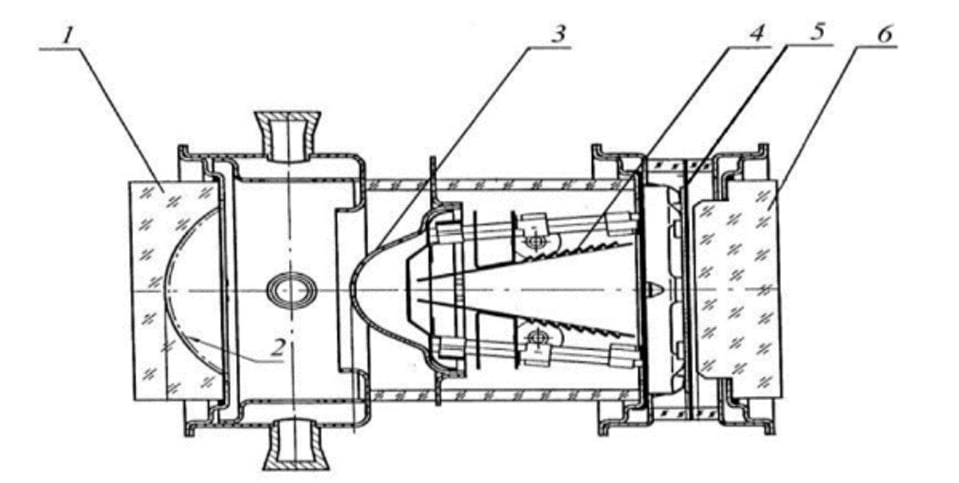
\includegraphics[width=0.7\linewidth]{ваки_2_!.jpg}
    \caption{Схема внутреннего устройства ЭОП}
\end{figure}
 1 -- стекловолоконное входное окно,
 2 -- фотокатод,
 3 -- анод,
 4 -- отклоняющие пластины,
 5 -- микроканальная плата,
 6 -- выходное стекловолоконное окно
\\
\\
\textbf{Фотокатод} - химическая смесь, нанесенная на внутреннюю поверхность входного окна, покрытую тонкой полупрозрачной металлической пленкой.  
\\
\textbf{Микроканальная пластина} (МКП) представляет собой многоканальный электронный умножитель («сотовая» структура, образованная большим числом стеклянных каналов). Попадая в один из микроканалов, электрон ударяется о его стенки в результате чего происходит вторичная электронная эмиссия. Количество электронов возрастает, сигнал усиливается.
\\
\textbf{Люминисцентный экран} - экран, способный создавать свечение в видимом свете, при попадании на него электронов.


\subsection*{Где используется ЭОП:}
\begin{itemize}
    \item Приборы ночного видения
    \item ИК-камеры
    \item Медицина: эндоскопы, рентгеновские аппараты
    \item Астрономия, ядерные исследования, физика плазмы
\end{itemize}

\subsection*{Принцип действия}
Входное оптическое излучение попадает на фотокатод (ФК). Фотокатод испускает электроны,которые ускоряются в поле между катодом и анодом.
Сферическая форма фотокатода и специально подобранная форма анода образуют иммерсионную электронную линзу, которая формирует изображение поверхности катода во входной плоскости микроканальной пластины (МКП).
Поток электронов, усиленный МКП, ускоряется в промежутке между выходной плоскость МКП и экраном. Экран покрыт люминофором, который при электронном возбуждении обеспечивает свечение в зеленой области видимого спектра. Изображение на экране регистрируется с помощью видеокамеры. Прибор часто используется при работе с малым излучением.

\begin{figure}[htb]
    \centering
    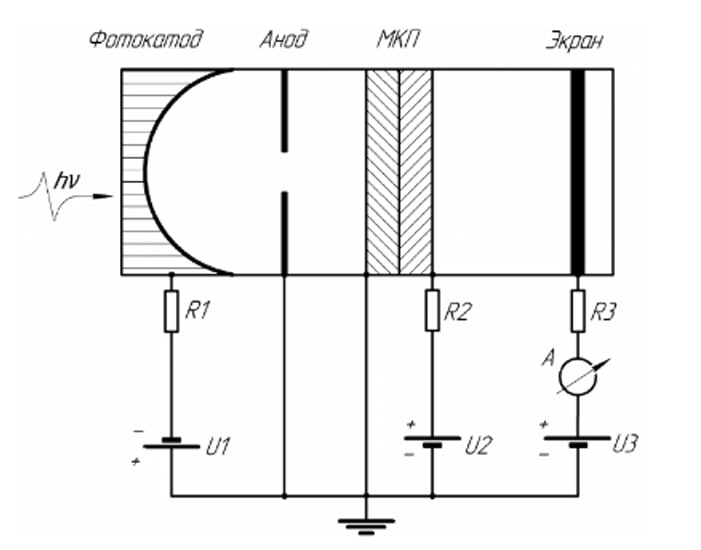
\includegraphics[width=0.7\linewidth]{ваки_2_2.jpg}
    \caption{Электрическая схема подключения ЭОП}
\end{figure}

% \subsection*{Основные формулы}
% Итоговый ток на катоде:
%     \begin{equation}
%  I_{\text{катод}}^\Sigma = I_{\text{катод}} - I_{\text{катод}}^0 \qquad (1)
%         \label{formula_I_cathode}
%     \end{equation}
% Коэффициент усиления МКП:
%     \begin{equation}
%  k = \frac{I_{\text{экран}}}{I_{\text{катод}}^\Sigma} \qquad (2)
%         \label{formula_k_I}
%     \end{equation}

%     \begin{equation}
%         \langle B_{\text{отн}}\rangle = \langle B_{\text{центр}}\rangle - \langle B_{\text{фон}}\rangle  \qquad (3)
%         \label{formula_B}
%     \end{equation}

%     \begin{equation}
%         \frac{B_i}{k_i} = \frac{B_1}{k_1}\ \ \Rightarrow \ \ k_i = B_i \frac{k_1}{B_1} \equiv \alpha B_i,\ \text{где}\ \alpha = \frac{k_1}{B_1} = \frac{4,393}{6,863} = 0,64 \qquad (4)
%         \label{formula_k_B}
%     \end{equation}



\section*{Ход работы}
\subsection*{Измерение зависимости коэффициента усиления МКП от напряжения}

Для проверки работы системы был включён источник света и на камере получено изображение решётки:

\begin{figure}[H]
    \centering
    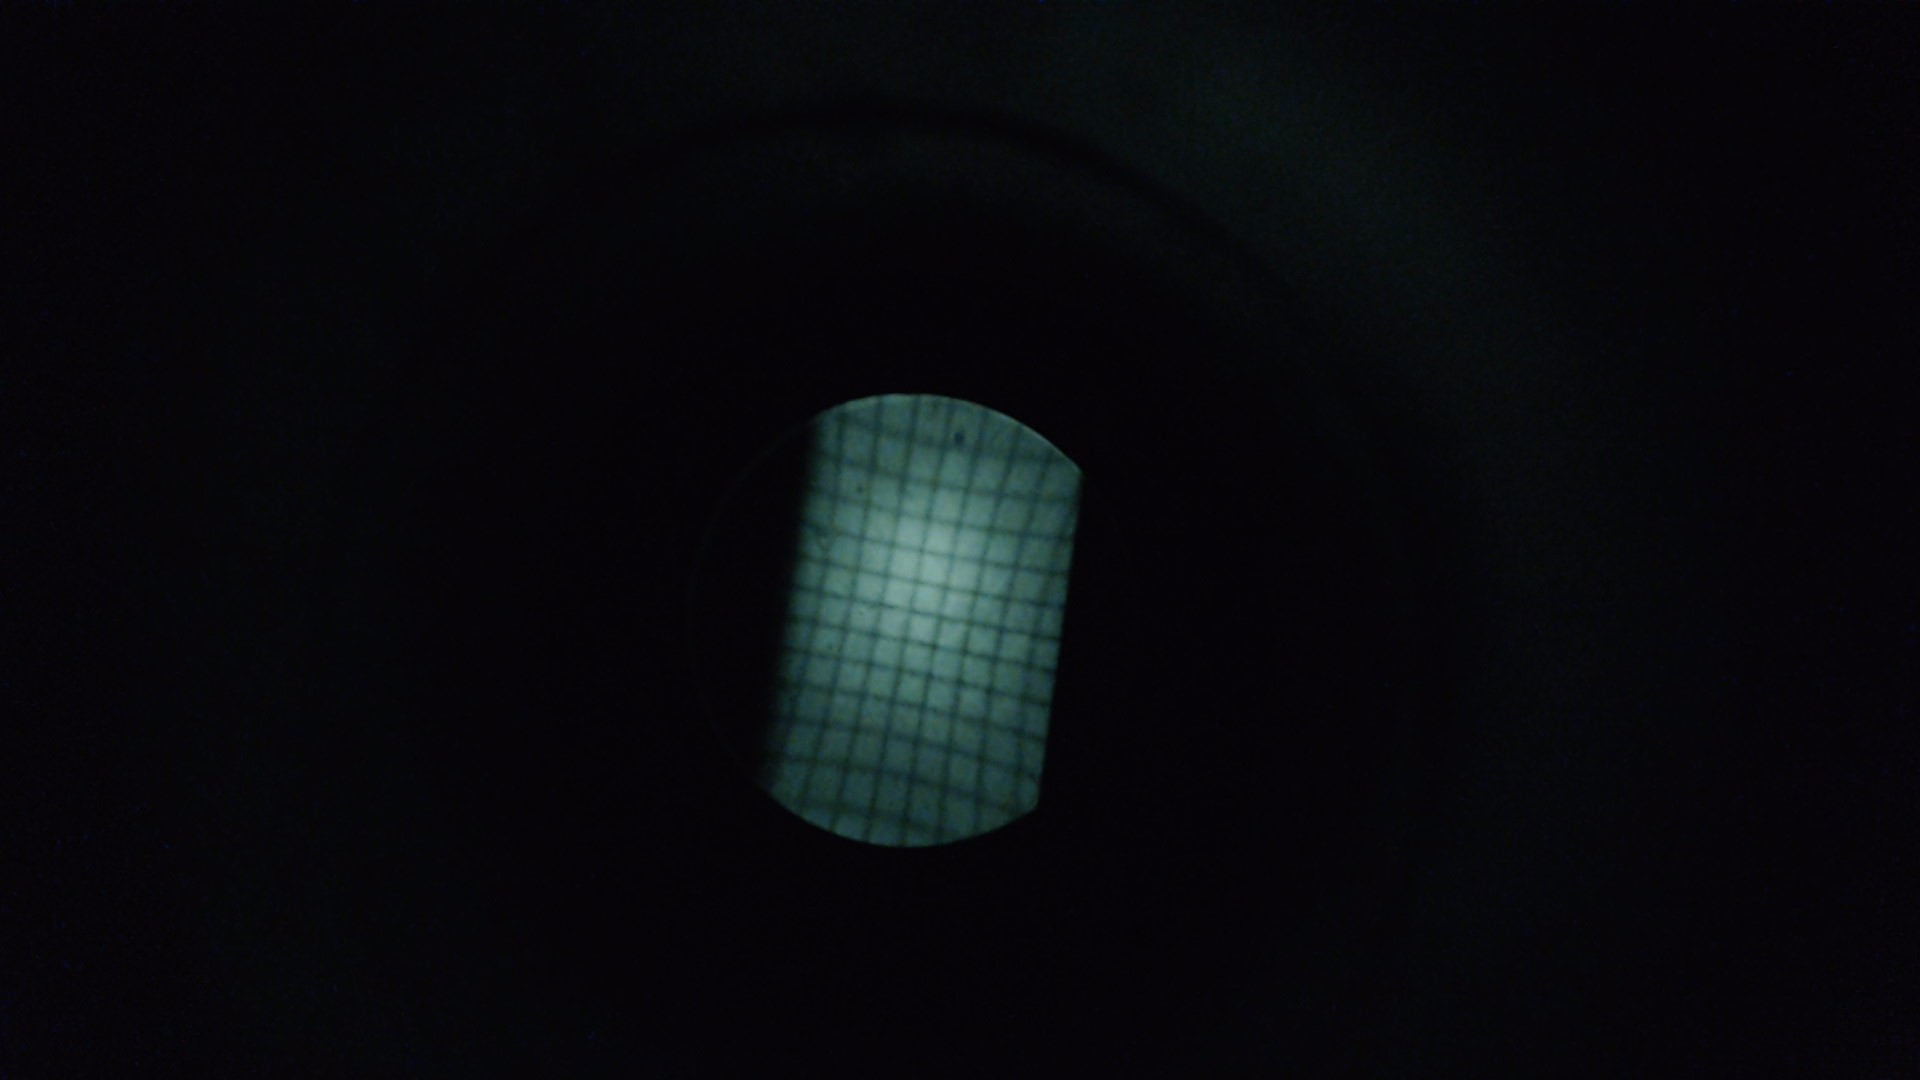
\includegraphics[width=1\linewidth]{Решётка.jpg}
    \caption{Полученное изображение решётки}
\end{figure}

На катоде было зафиксировано напряжение 2,9367 кВ, на экране 3,0041 кВ. При нулевом напржении на МКП появился теневой ток $I_{\text{темн}} = 0,01297$ мкА, возникающий из-за внешних воздействий на пластинку и ЭОП в целом, например, из-за термоэлектронной эмиссии.
Коэффициент усиления МКП $\alpha$ определяется отношением выходного тока (тока экрана) к входному току (току катода), с условием вычитания темнового тока.
Получается зависимость коэффициента усиления от напряжения:
\[ \alpha = \dfrac{I_{\text{экр}}}{I_{\text{кат}} - I_{\text{тен}}} \]

Была проведена серия измерений для получения зависимости тока катода от напряжения МКП. Результаты представлены в таблице 1. На рисунке 4 изображён график зависимости натурального логарифма от напряжении на МКП. Видно, что точки хорошо аппроксимируются линейной зависимость.


% Проведём серию измерений. Будем при различных значениях напряжения на микроканальной пластине измерять ток на катоде и ток на экране. Ток на экране будет больше тока на катоде, поскольку микроканальная пластина "умножила"\ падающие на нее электроны.
% Соответственно, коэффициент усиления -- то, во сколько раз ток после пластины стал больше -- вычисляется по формуле (2). Однако, из-за особенностей проектирования установки ток на катоде будет ненулевым, даже если фотоны не падают на фотокатод.
% Значит, закроем входное отверстие установки, чтобы в неё не попадал свет, и измерим нулевой ток на катоде $I_{\text{катод}}^0$ (при различных $U_{\text{мкп}}$).
% Отнормируем на эту величину значения токов на катоде (формула (1)), получившуюся величину обозначим $I_{\text{катод}}^\Sigma$. Итоговые результаты измерений представлены в таблице \ref{table_multi_coef}.

\begin{table}[H]
\centering
\begin{tabular}{|c|c|c|c|}
\hline
$I_{\text{кат}}$   & $U_{\text{МКП}}$  & $I_{\text{экр}}$   & $\alpha$   \\ \hline
0,01447 & 0,5785 & 0,048   & 32,000    \\ \hline
0,01434 & 0,6909 & 0,33692 & 245,927  \\ \hline
0,01476 & 0,7896 & 1,30269 & 727,7598 \\ \hline
0,01489 & 0,6295 & 0,12337 & 64,25521 \\ \hline
0,01523 & 0,7409 & 0,76294 & 337,5841 \\ \hline
0,01485 & 0,6530  & 0,18682 & 99,37234 \\ \hline
0,01506 & 0,7500   & 0,86399 & 413,3923 \\ \hline
\end{tabular}
\caption{Измерения без фильтров}
\end{table}

\begin{figure}[H]
    \centering
    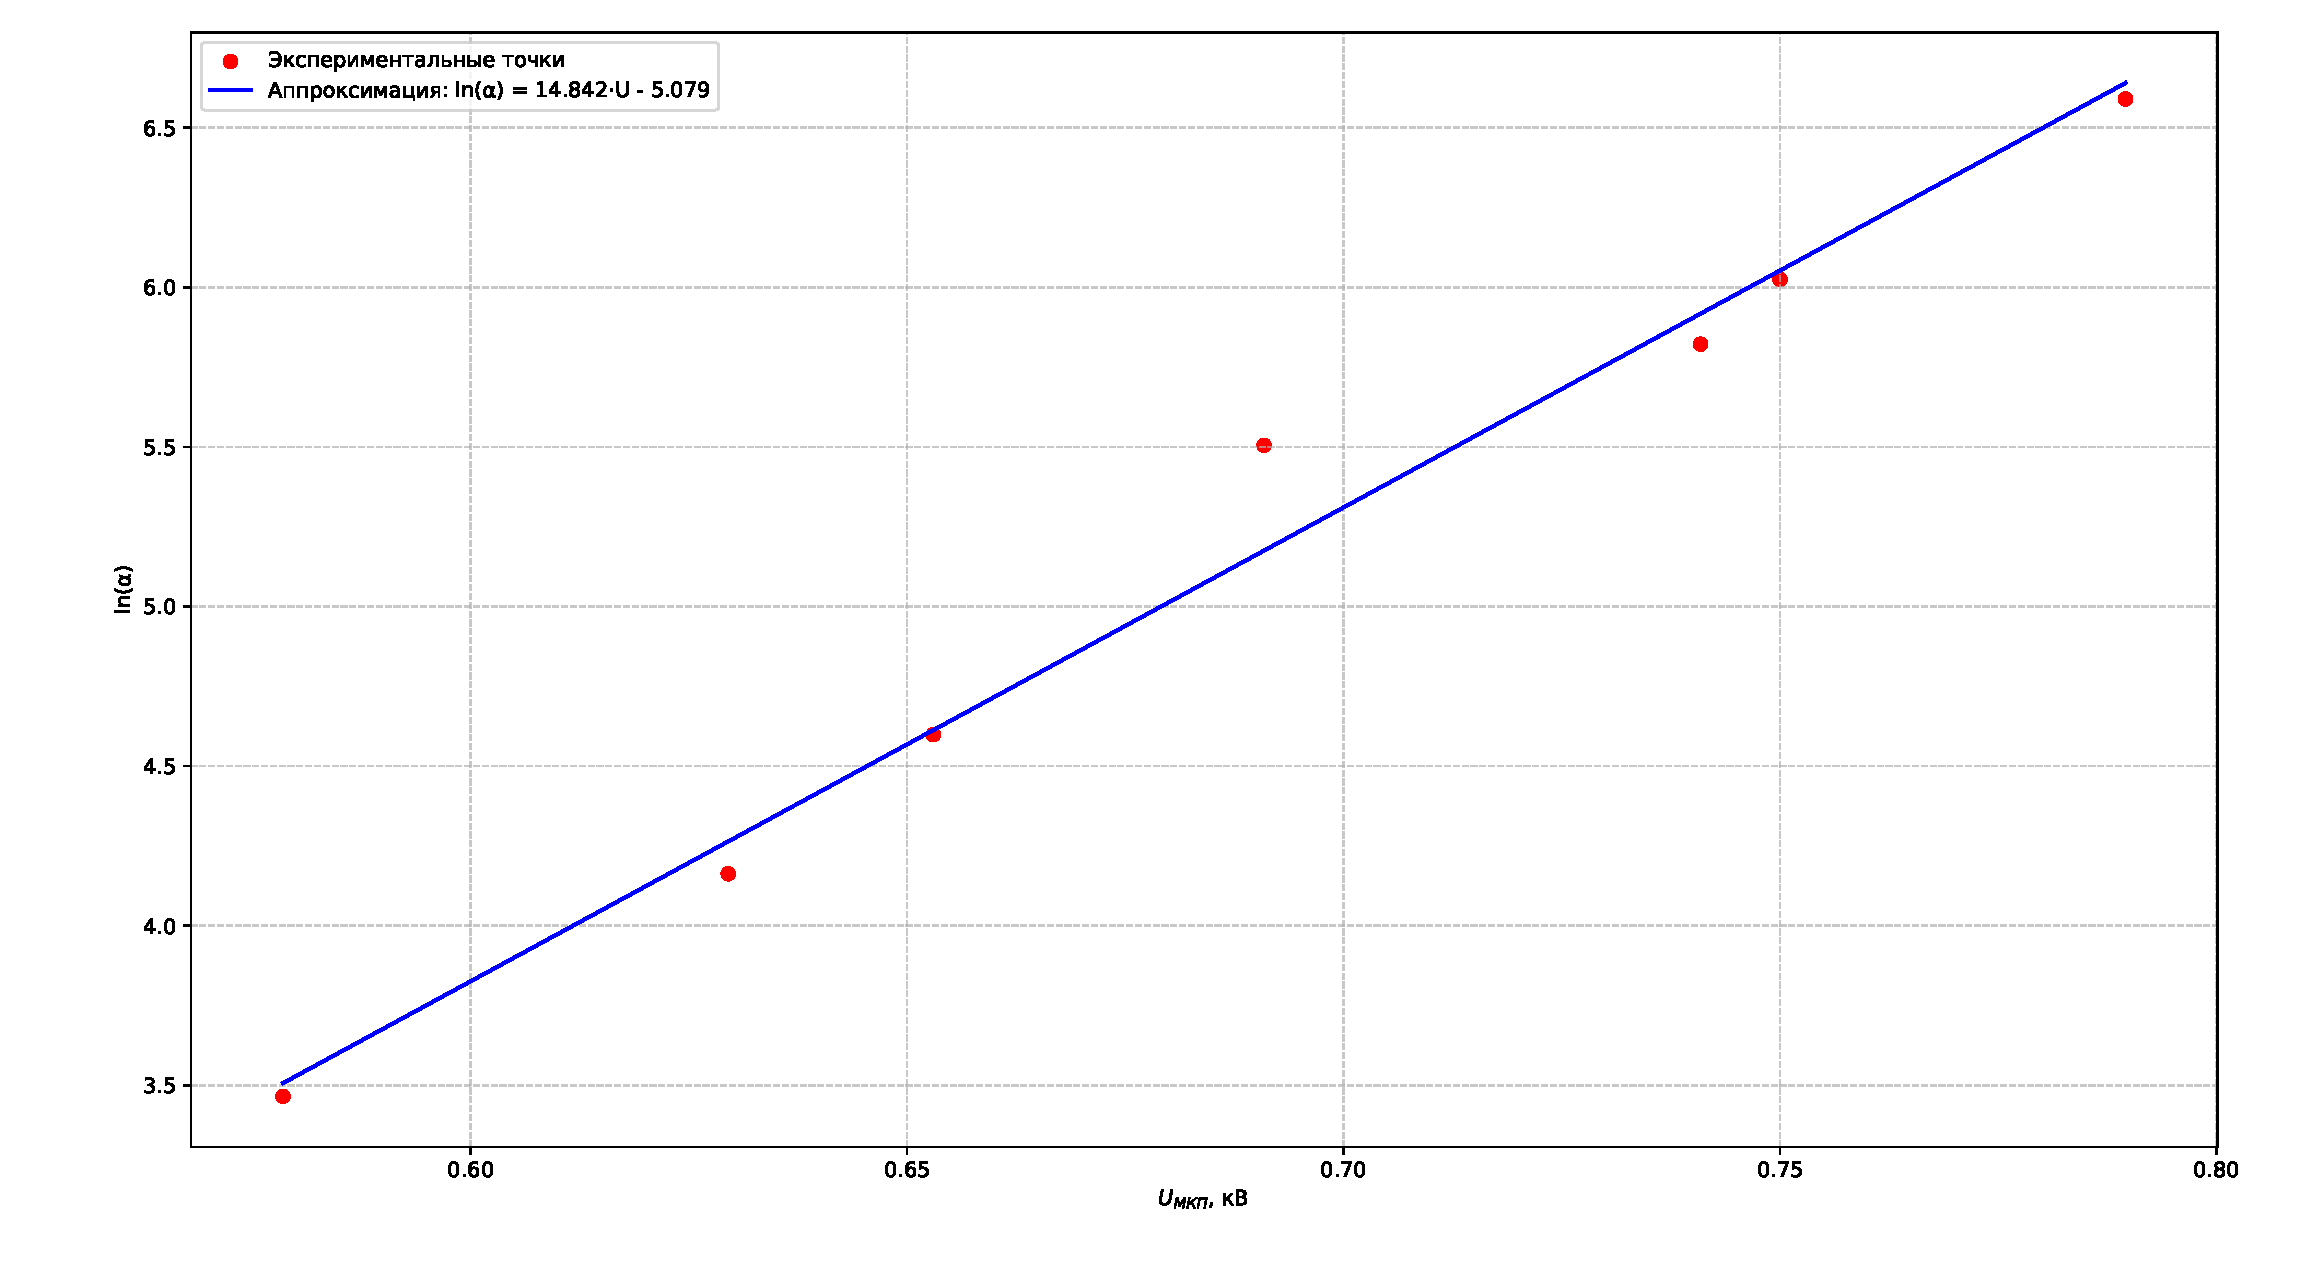
\includegraphics[width=1\linewidth]{a(U).pdf}
    \caption{График зависимости $\ln(\alpha)(U_{\text{МКП}})$}
\end{figure}

Аналогичные серии измерений были проведены для изображений, полученных с одним и двумя примерно одинаковыми фильтрами. Результаты представлены в таблице 2, на рисунке 5 изображены графики зависимостей логарифма тока на экране от напряжения на МКП.

\begin{table}[H]
\centering
\begin{tabular}{|c|c|c|c|c|c|}
\hline
\multicolumn{3}{|c|}{Один фильтр} & \multicolumn{3}{c|}{Два фильтра} \\ \hline
$I_{\text{кат}}$   & $U_{\text{МКП}}$  & $I_{\text{экр}}$   & $I_{\text{кат}}$   & $U_{\text{МКП}}$  & $I_{\text{экр}}$ \\ \hline
0,00089 & 0,7484 & 0,05213 & 0,00109 & 1,0395 & 0,06863 \\ \hline
0,00108 & 0,7914 & 0,09772 & 0,00126 & 1,0939 & 0,11298 \\ \hline
0,0013  & 0,8624 & 0,26374 & 0,00136 & 1,1282 & 0,14665 \\ \hline
0,00135 & 0,8915 & 0,38008 & 0,00141 & 1,1524 & 0,17624 \\ \hline
0,00146 & 0,924  & 0,55774 & 0,00153 & 1,1735 & 0,2091  \\ \hline
0,00158 & 0,9567 & 0,79923 & 0,00162 & 1,2119 & 0,26504 \\ \hline
0,00166 & 0,9955 & 1,15334 & 0,0017  & 1,2314 & 0,30435 \\ \hline
0,00171 & 1,025  & 1,29432 & 0,0018  & 1,2651 & 0,36891 \\ \hline
0,00178 & 1,029  & 1,30269 & 0,00186 & 1,2719 & 0,39278 \\ \hline
0,00141 & 0,9227 & 0,61021 & 0,00199 & 1,285  & 0,4354  \\ \hline
0,00126 & 0,8557 & 0,25566 & 0,00189 & 1,2745 & 0,37703 \\ \hline
\end{tabular}
\caption{Измерения с одним и двумя фильтрами}
\end{table}

\begin{figure}[H]
    \centering
    
\includegraphics[width=1\linewidth]{I(U).pdf}
    \caption{График зависимости $\ln(I)(U_{\text{МКП}})$ для трёх серий измерений}
\end{figure}







\subsection*{Измерение спектральной чувствительности фотокатода}

\textbf{Спектральная чувствительность фотокатода} -- зависимость величины фототока от
спектрального состава падающего на катод излучения. Данная зависимость строится в
координатах $\lambda$ (длина волны) -- А/Вт или мА/Вт и показывает какой ток будет вырабатываться
фотокатодом при падении на него одного Вт мощности излучения заданной
длины волны.
При помощи разных фильтров были сняты зависимость интенсивности света от светодиода
в установке для разных цветов: красного (КС 10), синего (СС 4, СС 5), зелёного (ЗС 10), фиолетового (ФС 1), оранжевого (ДС 5) и пикми розового (ПС 7).

Так как у используемого спектрометра различная чувствительность к разным длинам волн, для
получения объективных данных необходимо домножить полученные спектры на калибровочные кривые.
На рисунках изображены откалиброванные графики спектров:


% \begin{figure}[H]
%     \centering
%     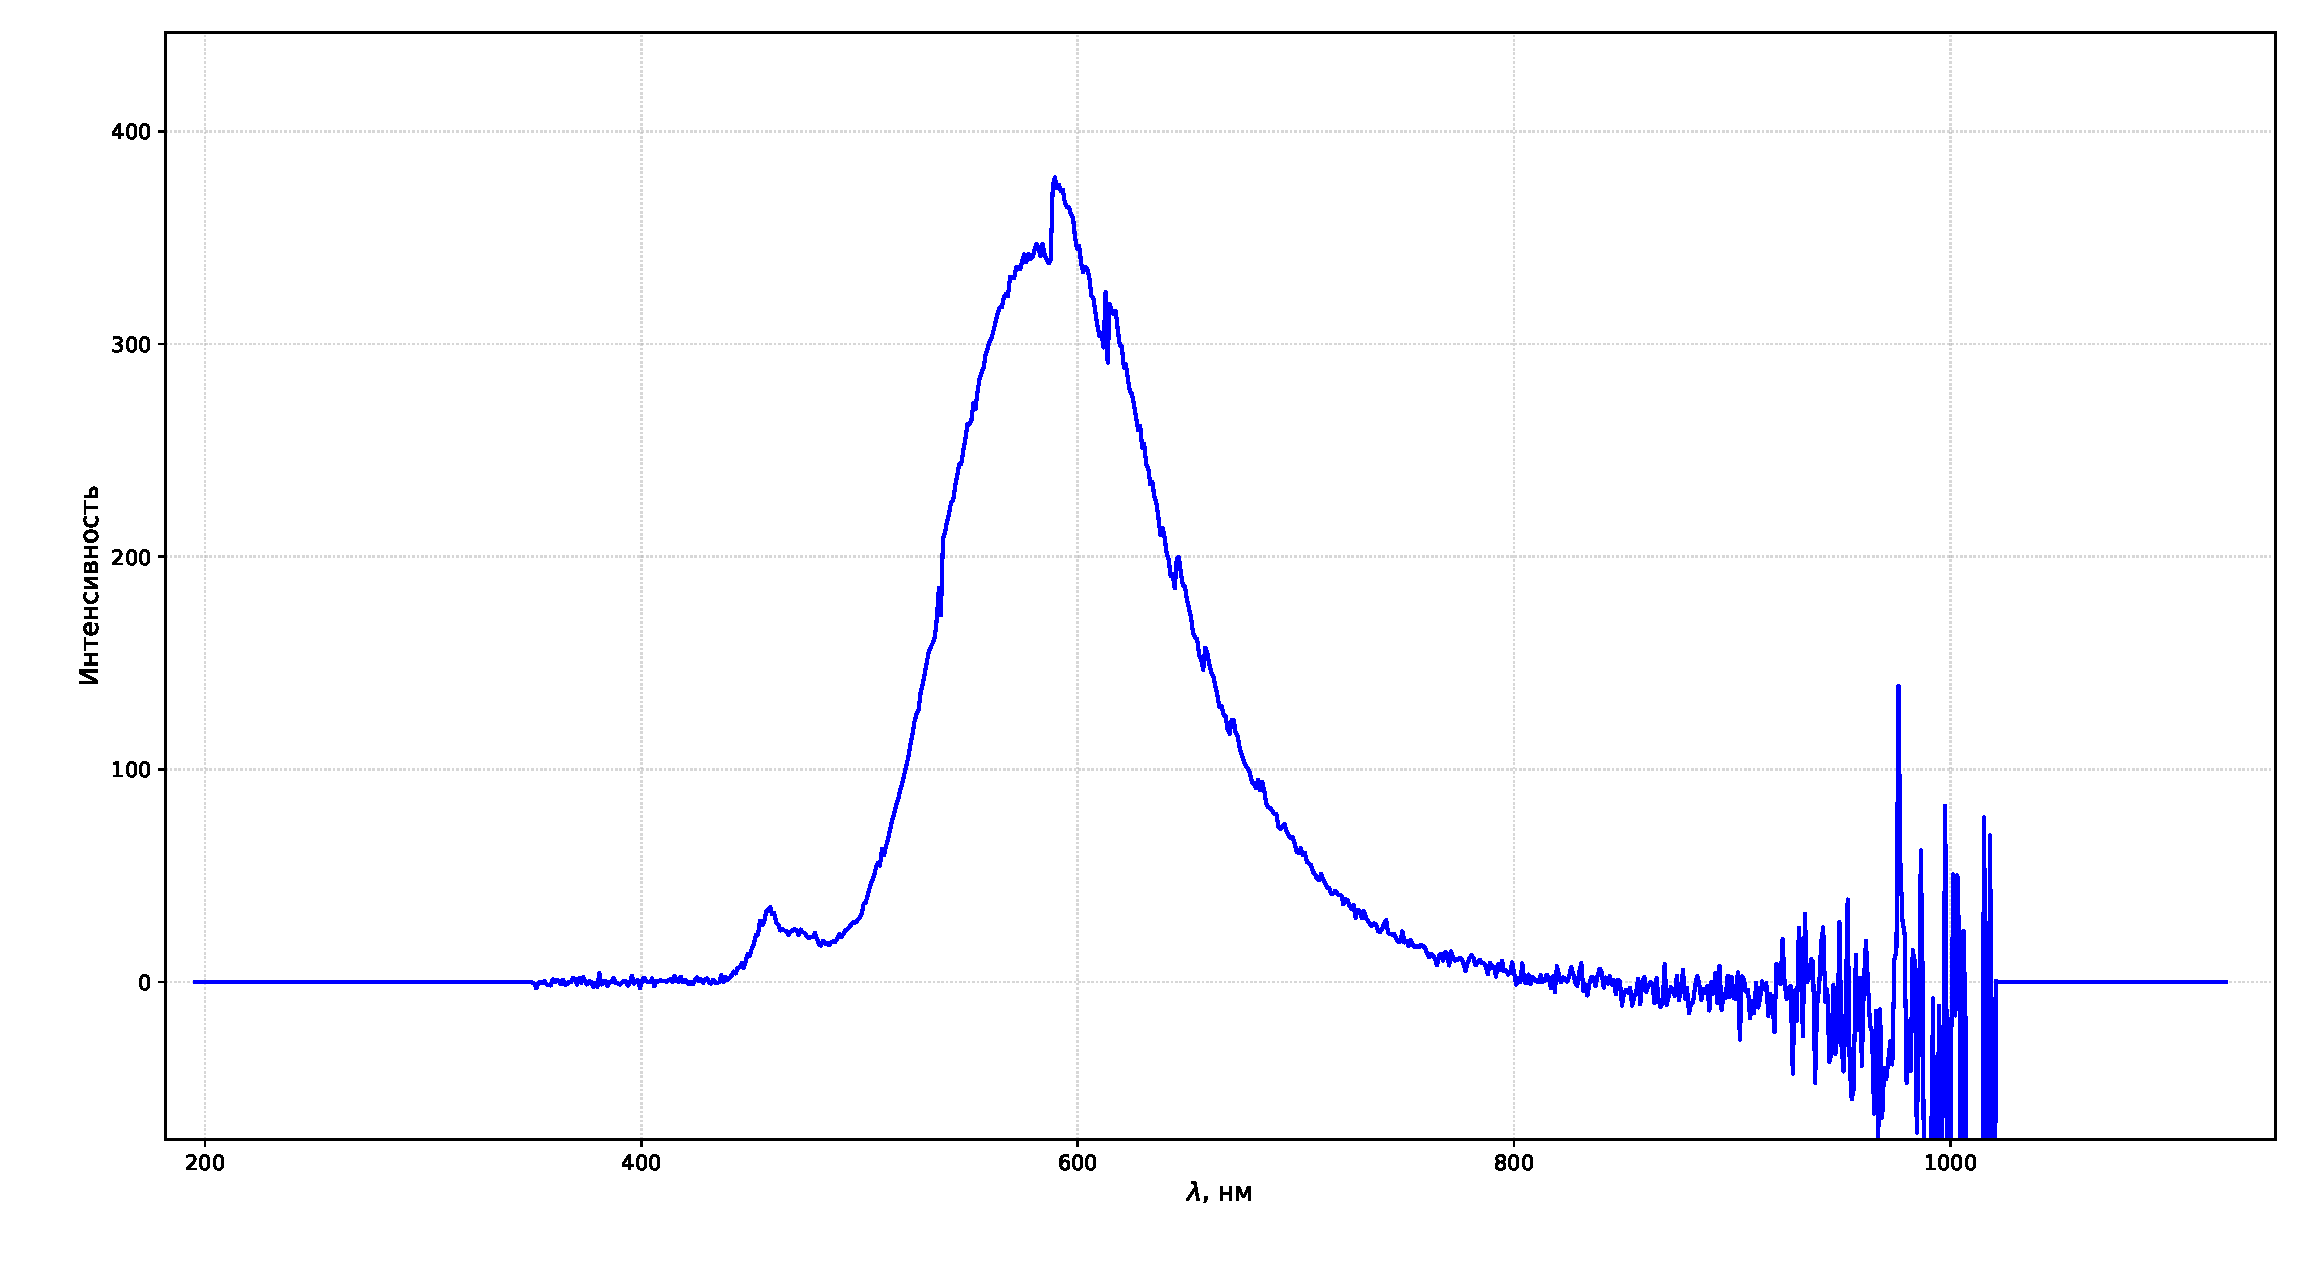
\includegraphics[width=1\linewidth]{ДС5.pdf}
%     \caption{Откалиброванный спектр фильтра ДС 5}
% \end{figure}

% \begin{figure}[H]
%     \centering
%     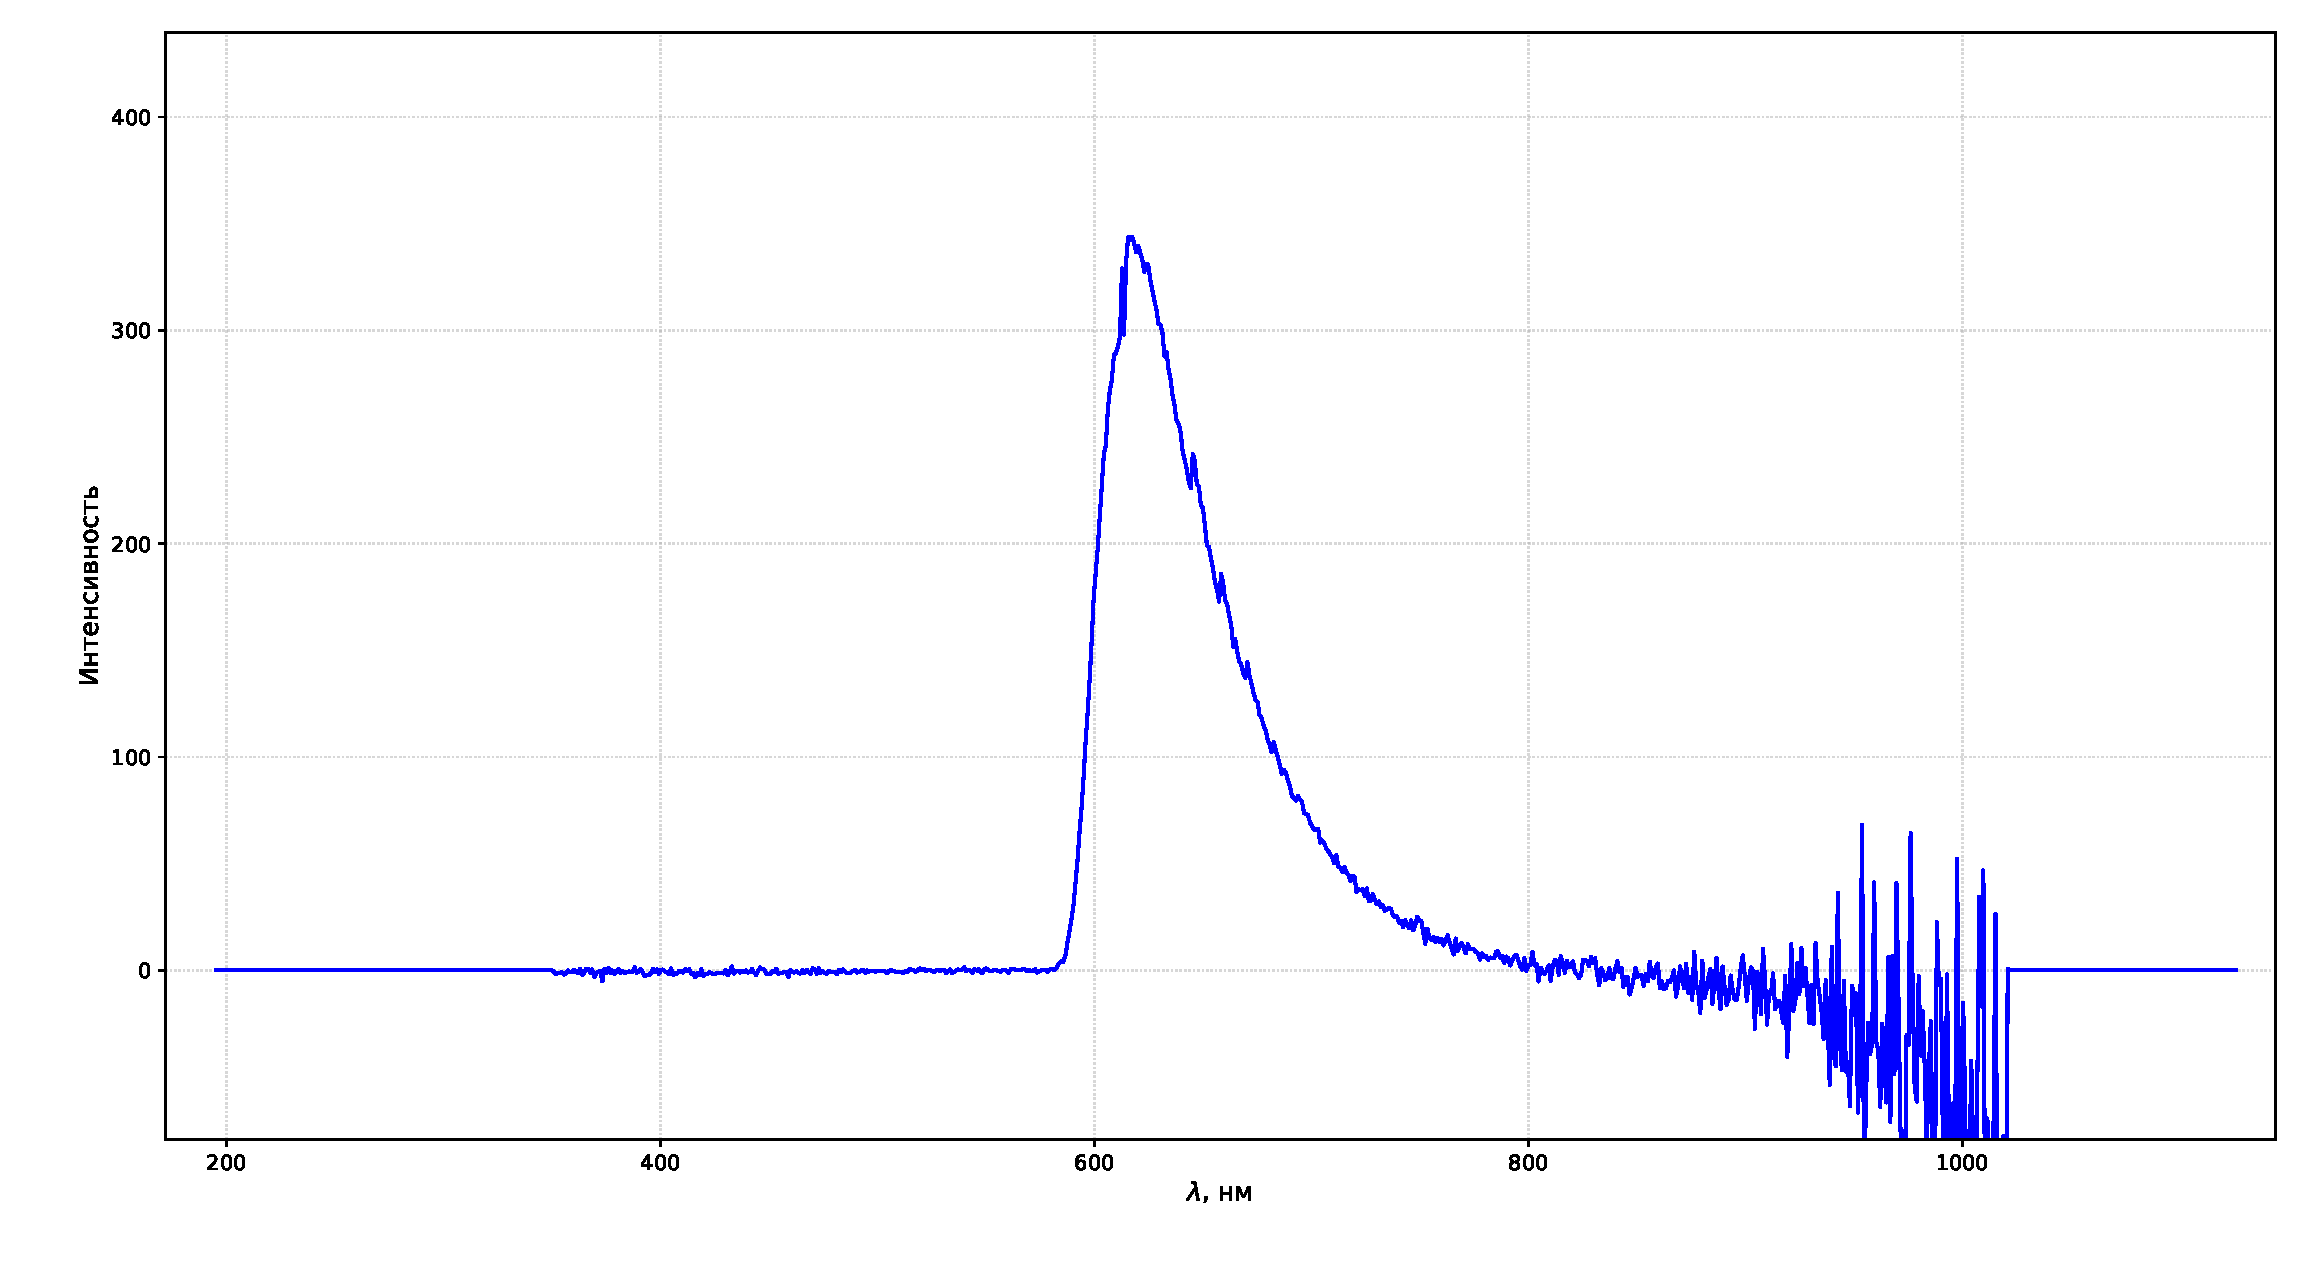
\includegraphics[width=1\linewidth]{КС10.pdf}
%     \caption{Откалиброванный спектр фильтра КС 10}
% \end{figure}

% \begin{figure}[H]
%     \centering
%     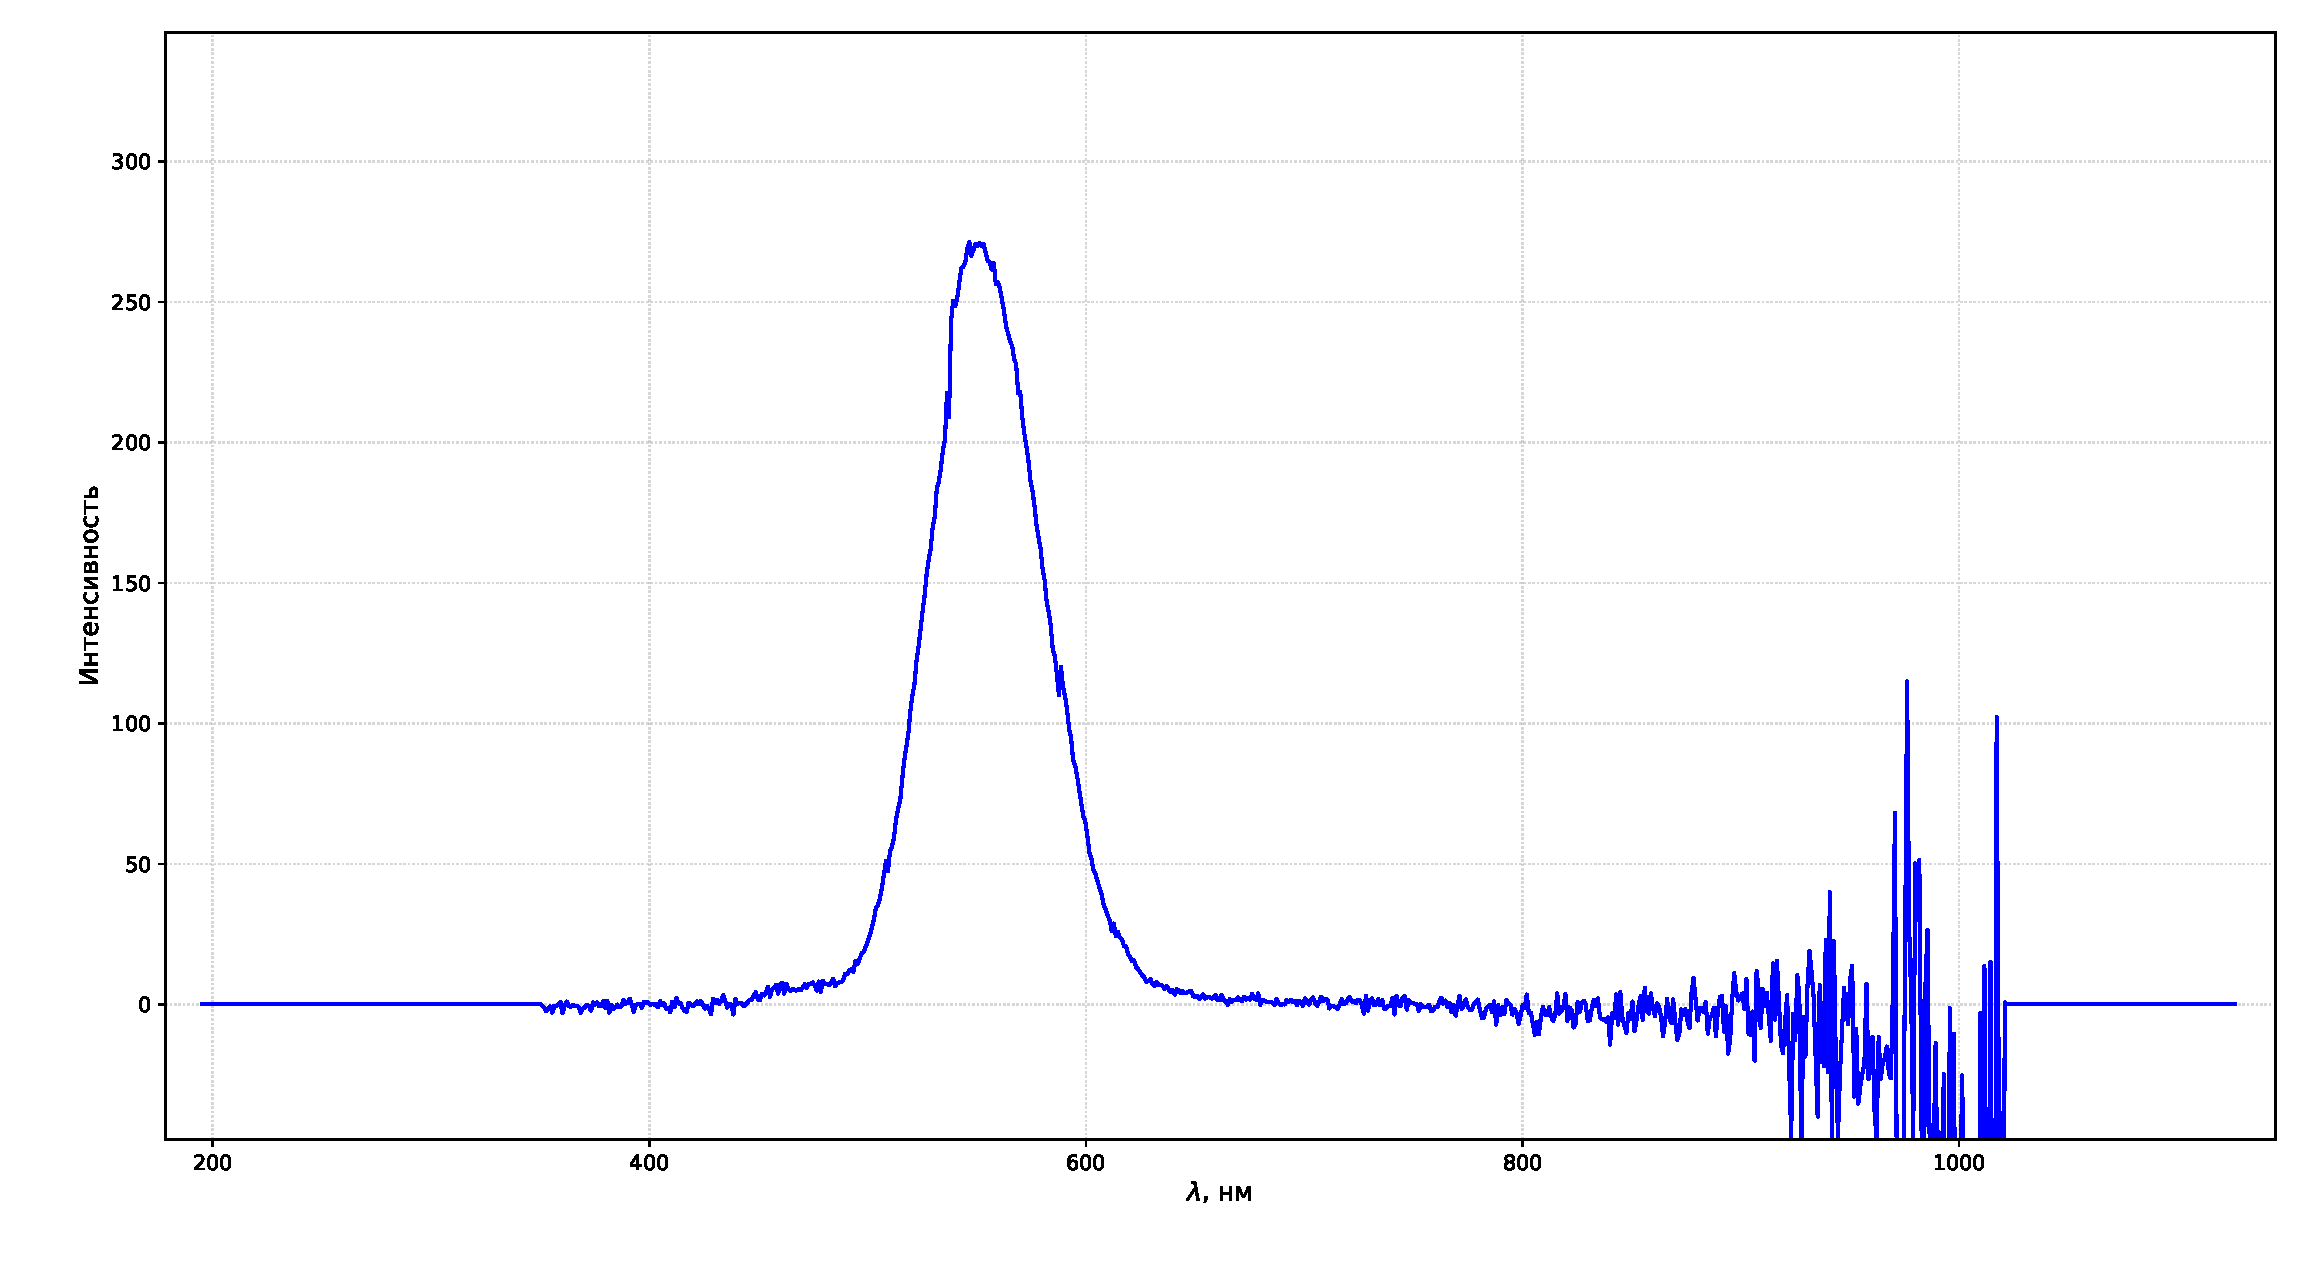
\includegraphics[width=1\linewidth]{ЗС10.pdf}
%     \caption{Откалиброванный спектр фильтра ЗС 10}
% \end{figure}

% \begin{figure}[H]
%     \centering
%     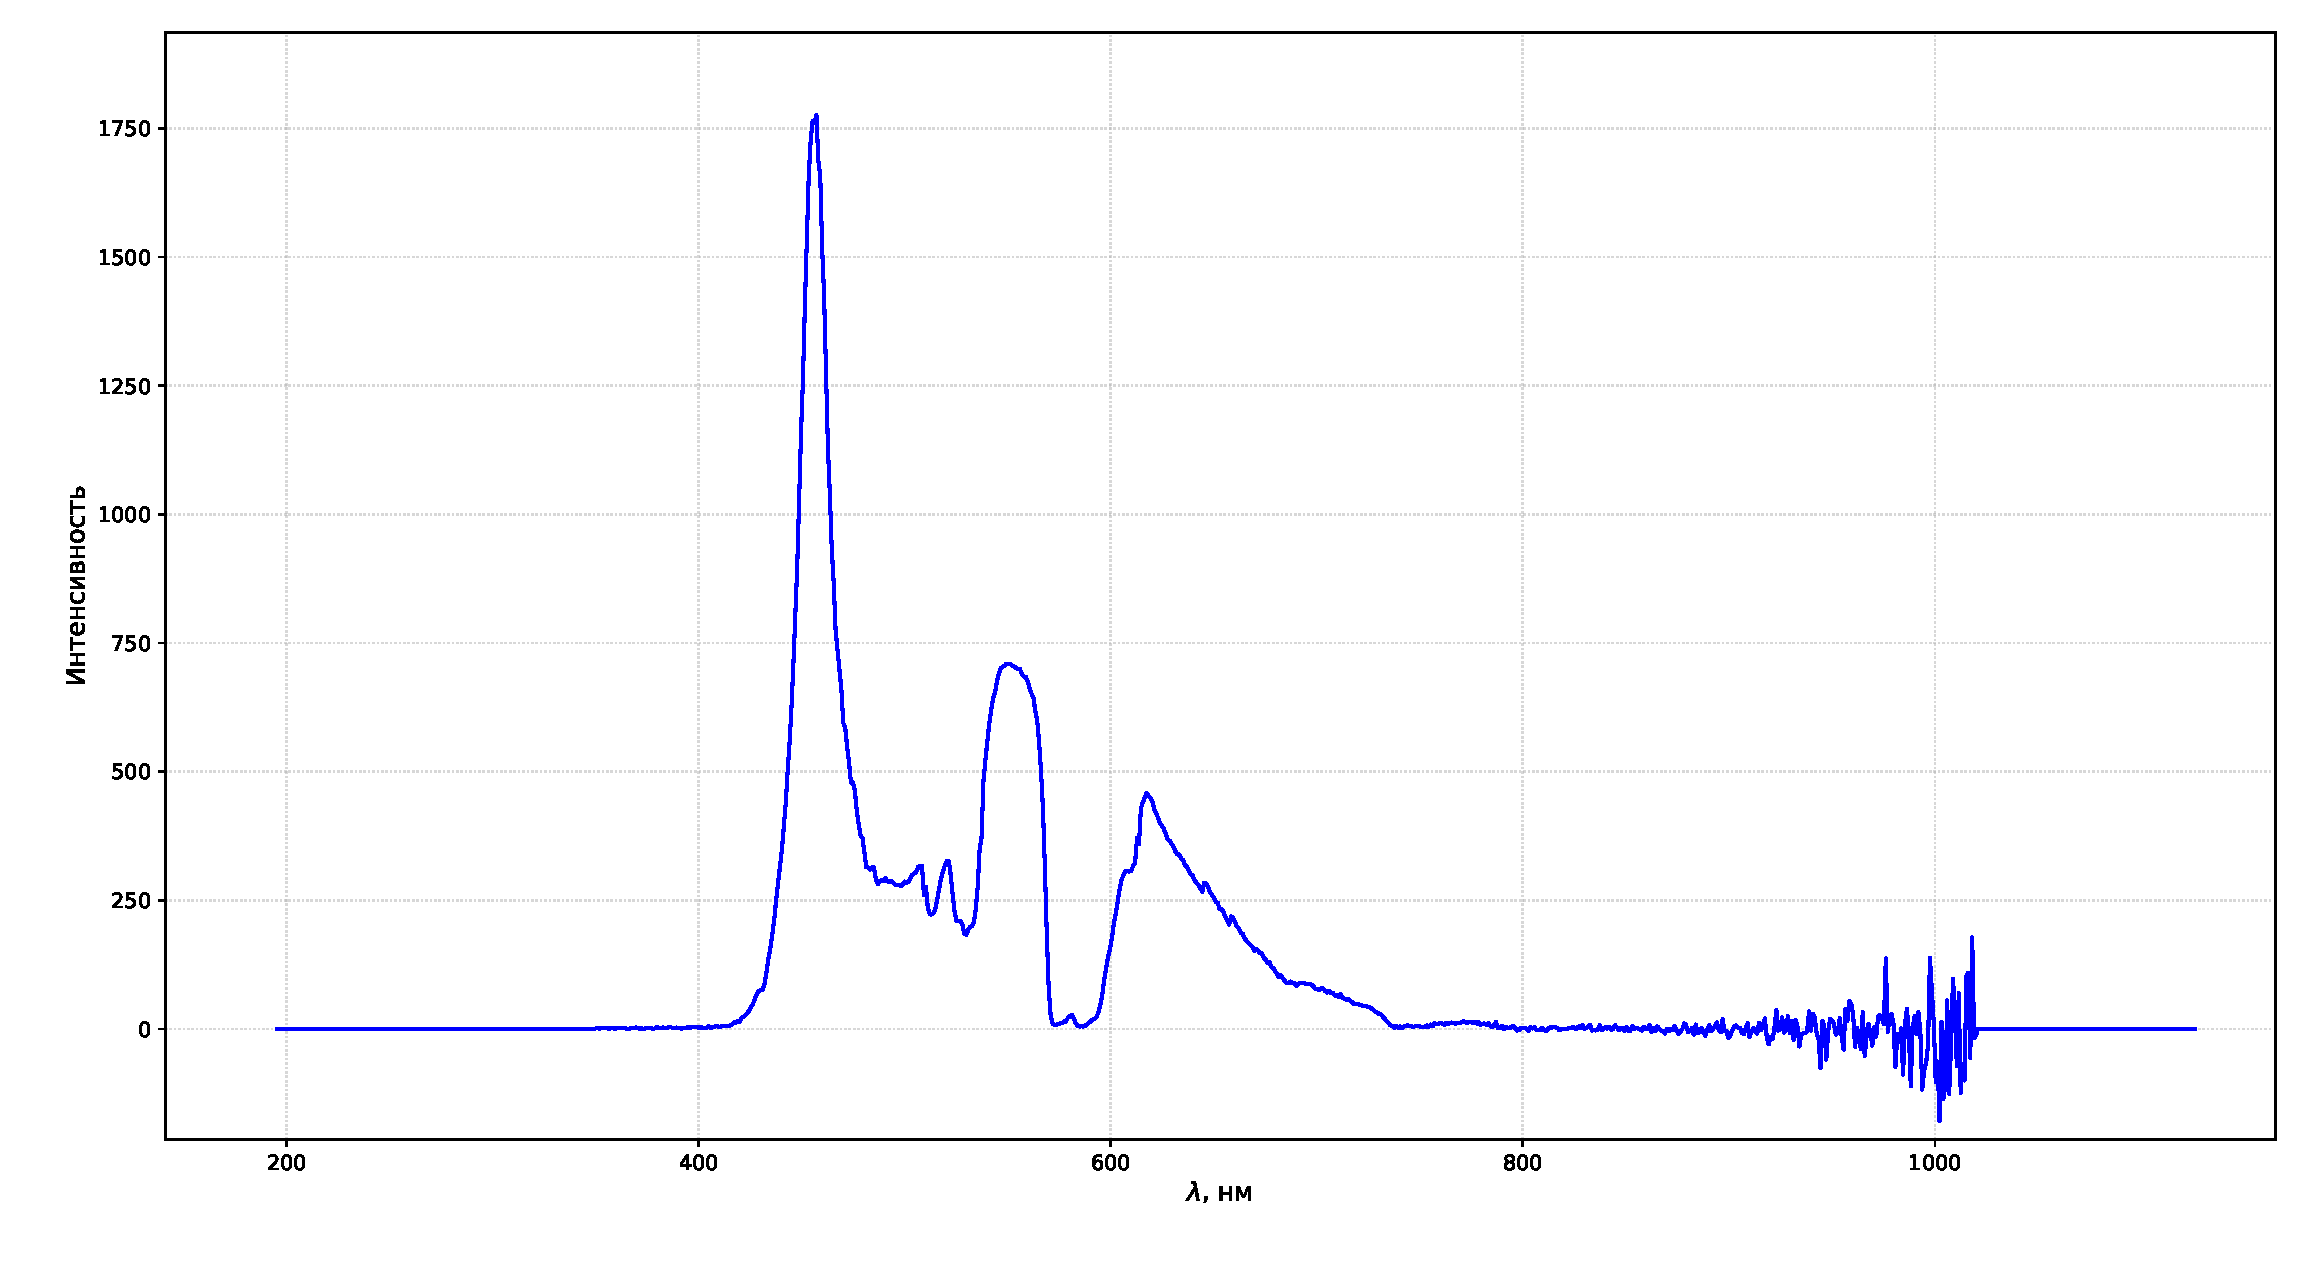
\includegraphics[width=1\linewidth]{ПС7.pdf}
%     \caption{Откалиброванный спектр фильтра ПС 7}
% \end{figure}

% \begin{figure}[H]
%     \centering
%     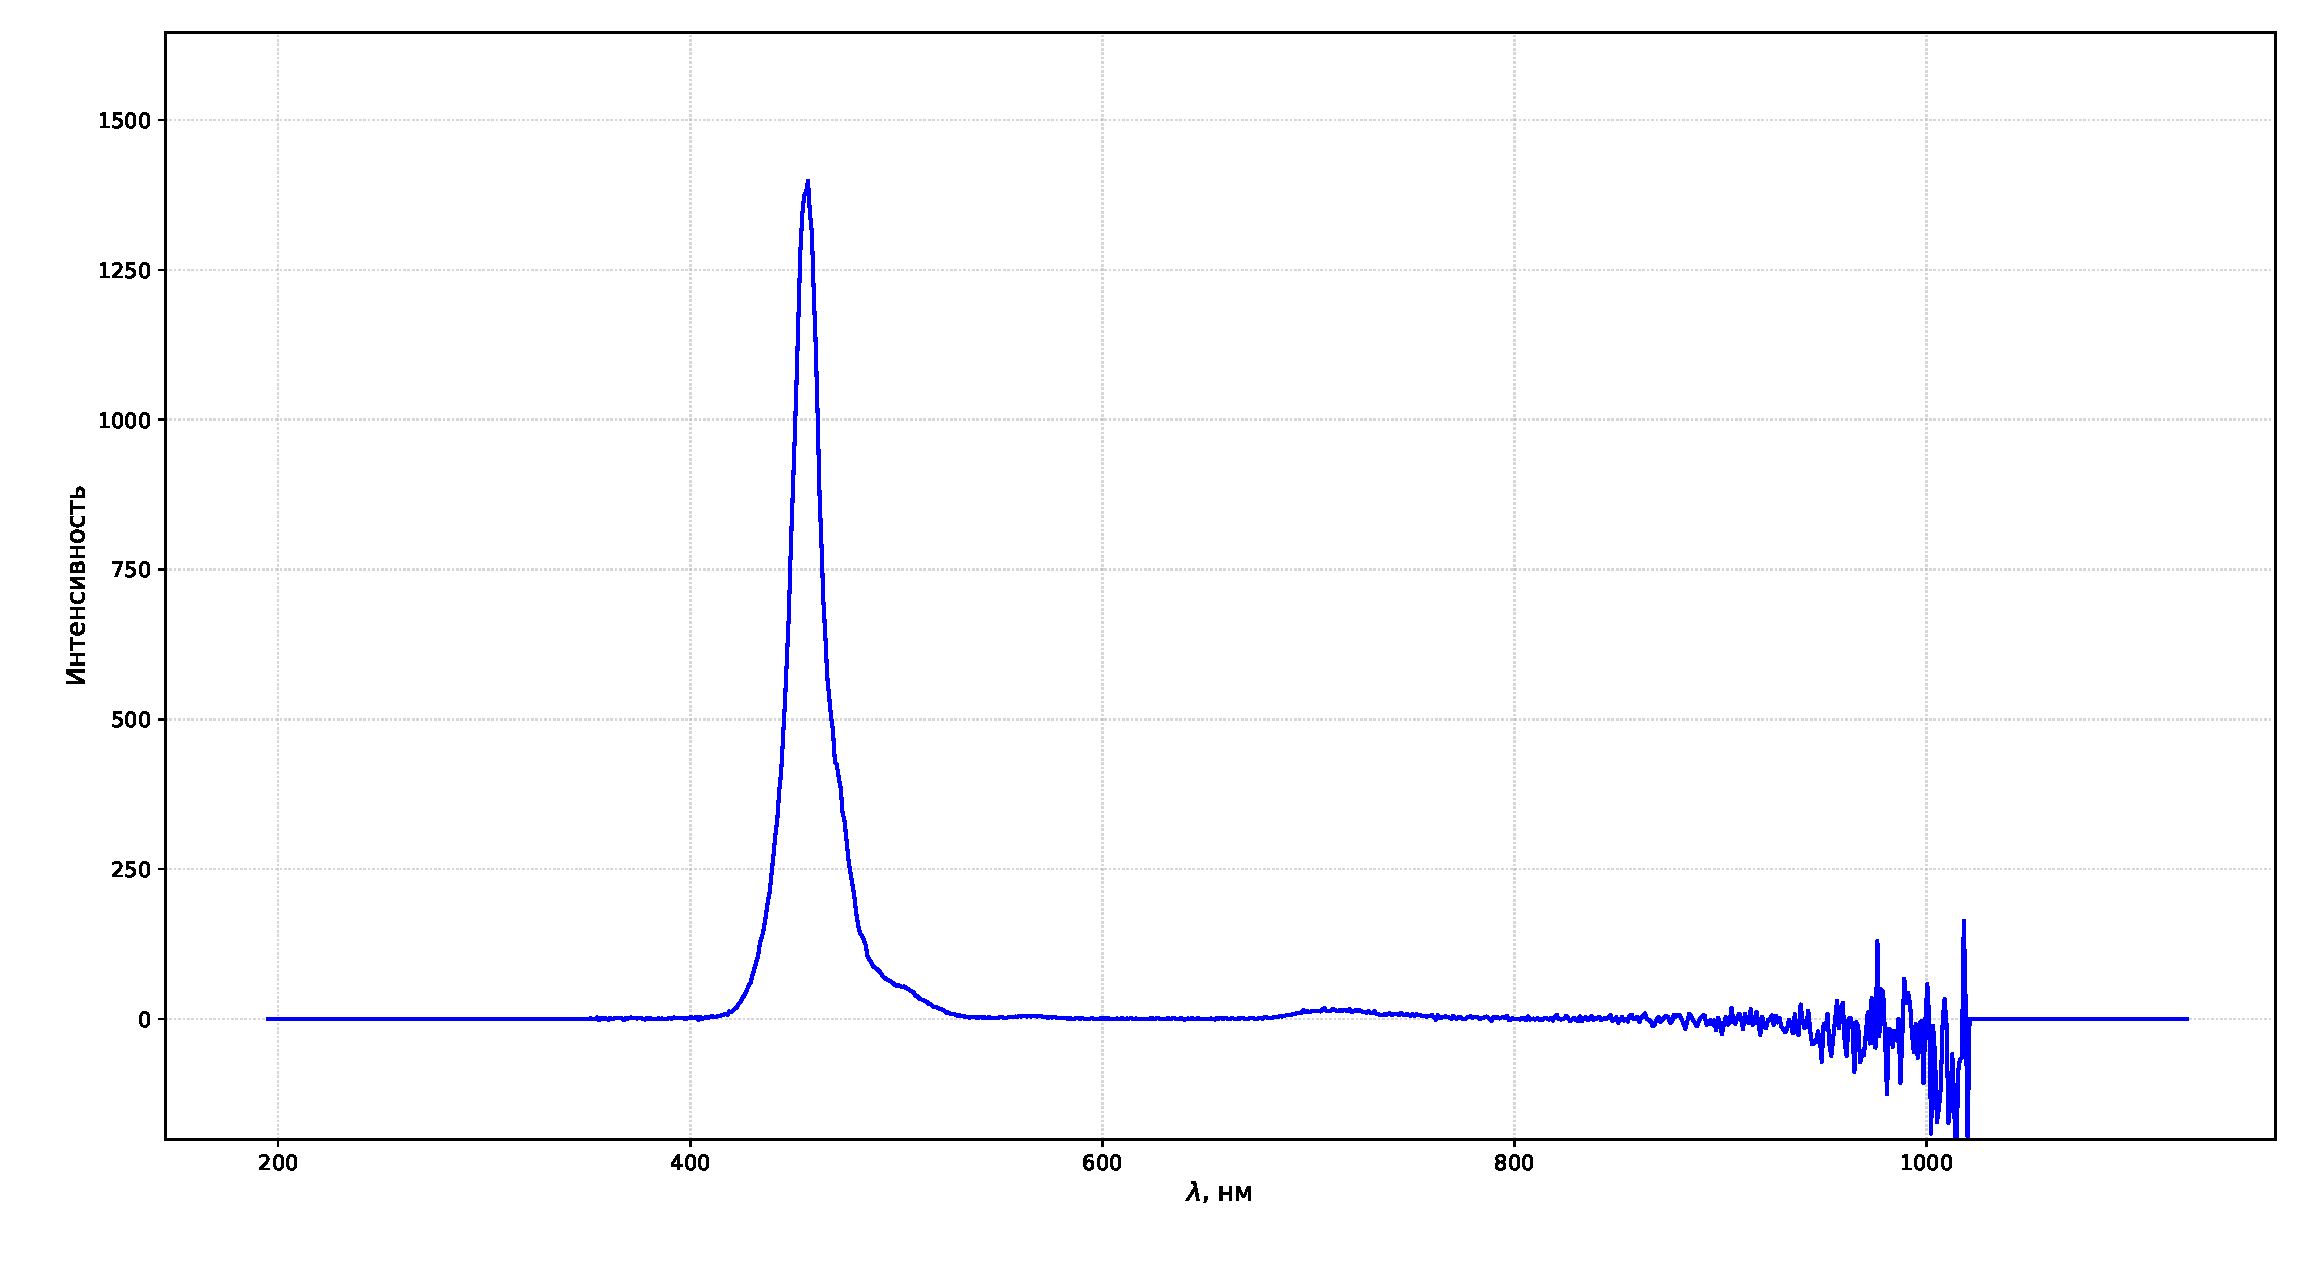
\includegraphics[width=1\linewidth]{СС5.pdf}
%     \caption{Откалиброванный спектр фильтра СС 5}
% \end{figure}

% \begin{figure}[H]
%     \centering
%     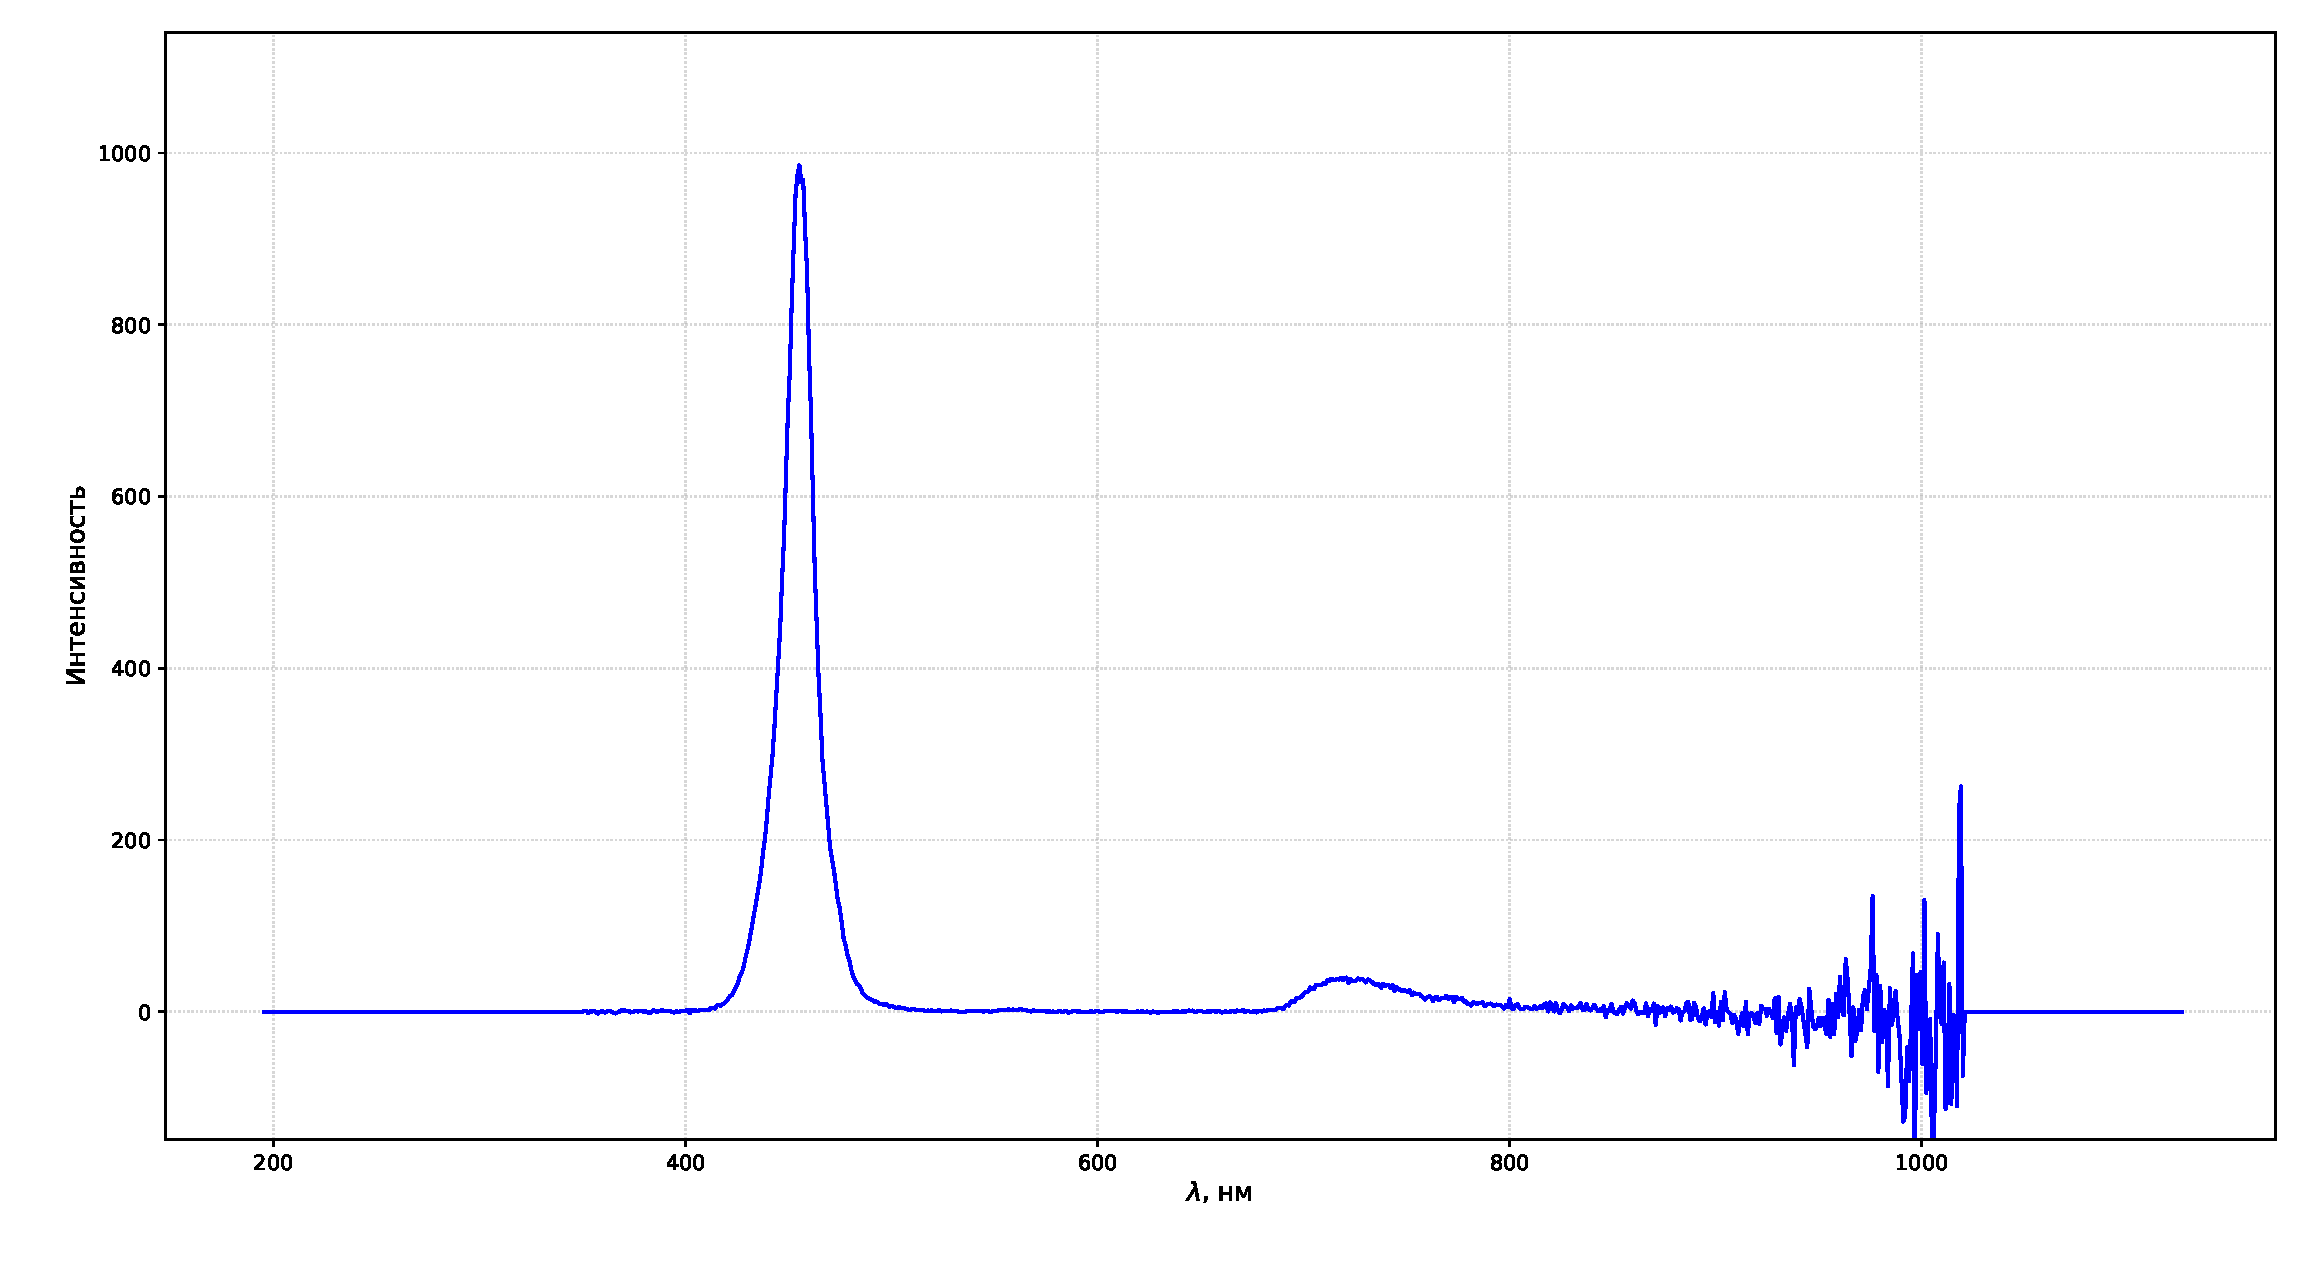
\includegraphics[width=1\linewidth]{СС4.pdf}
%     \caption{Откалиброванный спектр фильтра СС 4}
% \end{figure}

% \begin{figure}[H]
%     \centering
%     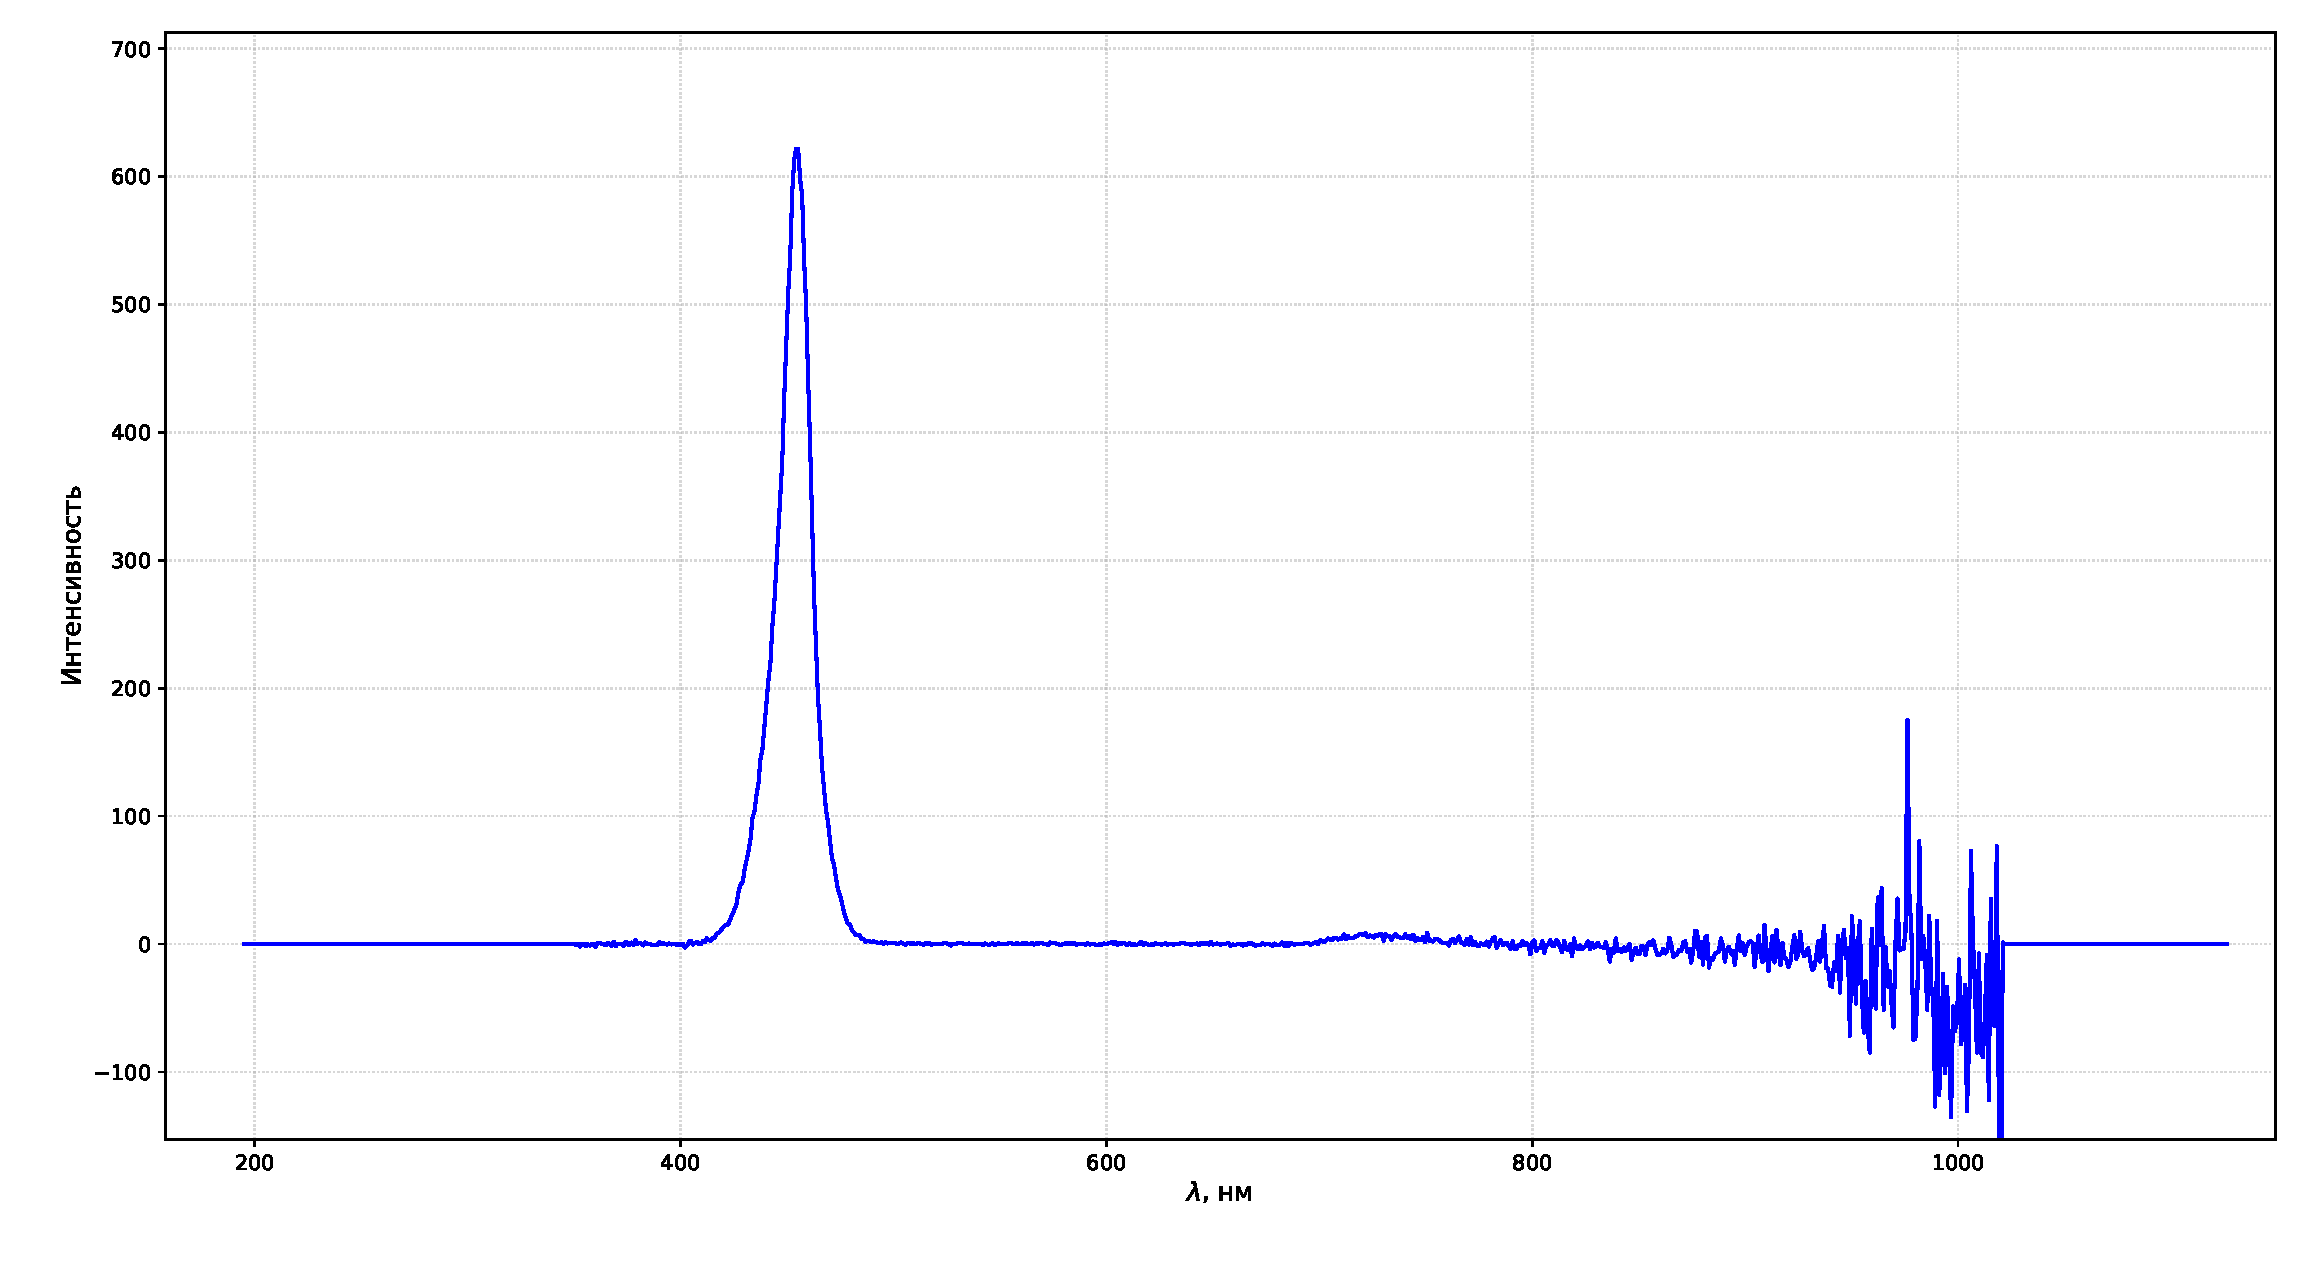
\includegraphics[width=1\linewidth]{ФС1.pdf}
%     \caption{Откалиброванный спектр фильтра ФС 1}
% \end{figure}


% Первая пара
\begin{figure}[H]
    \centering
    \begin{minipage}{0.48\textwidth}
        \centering
        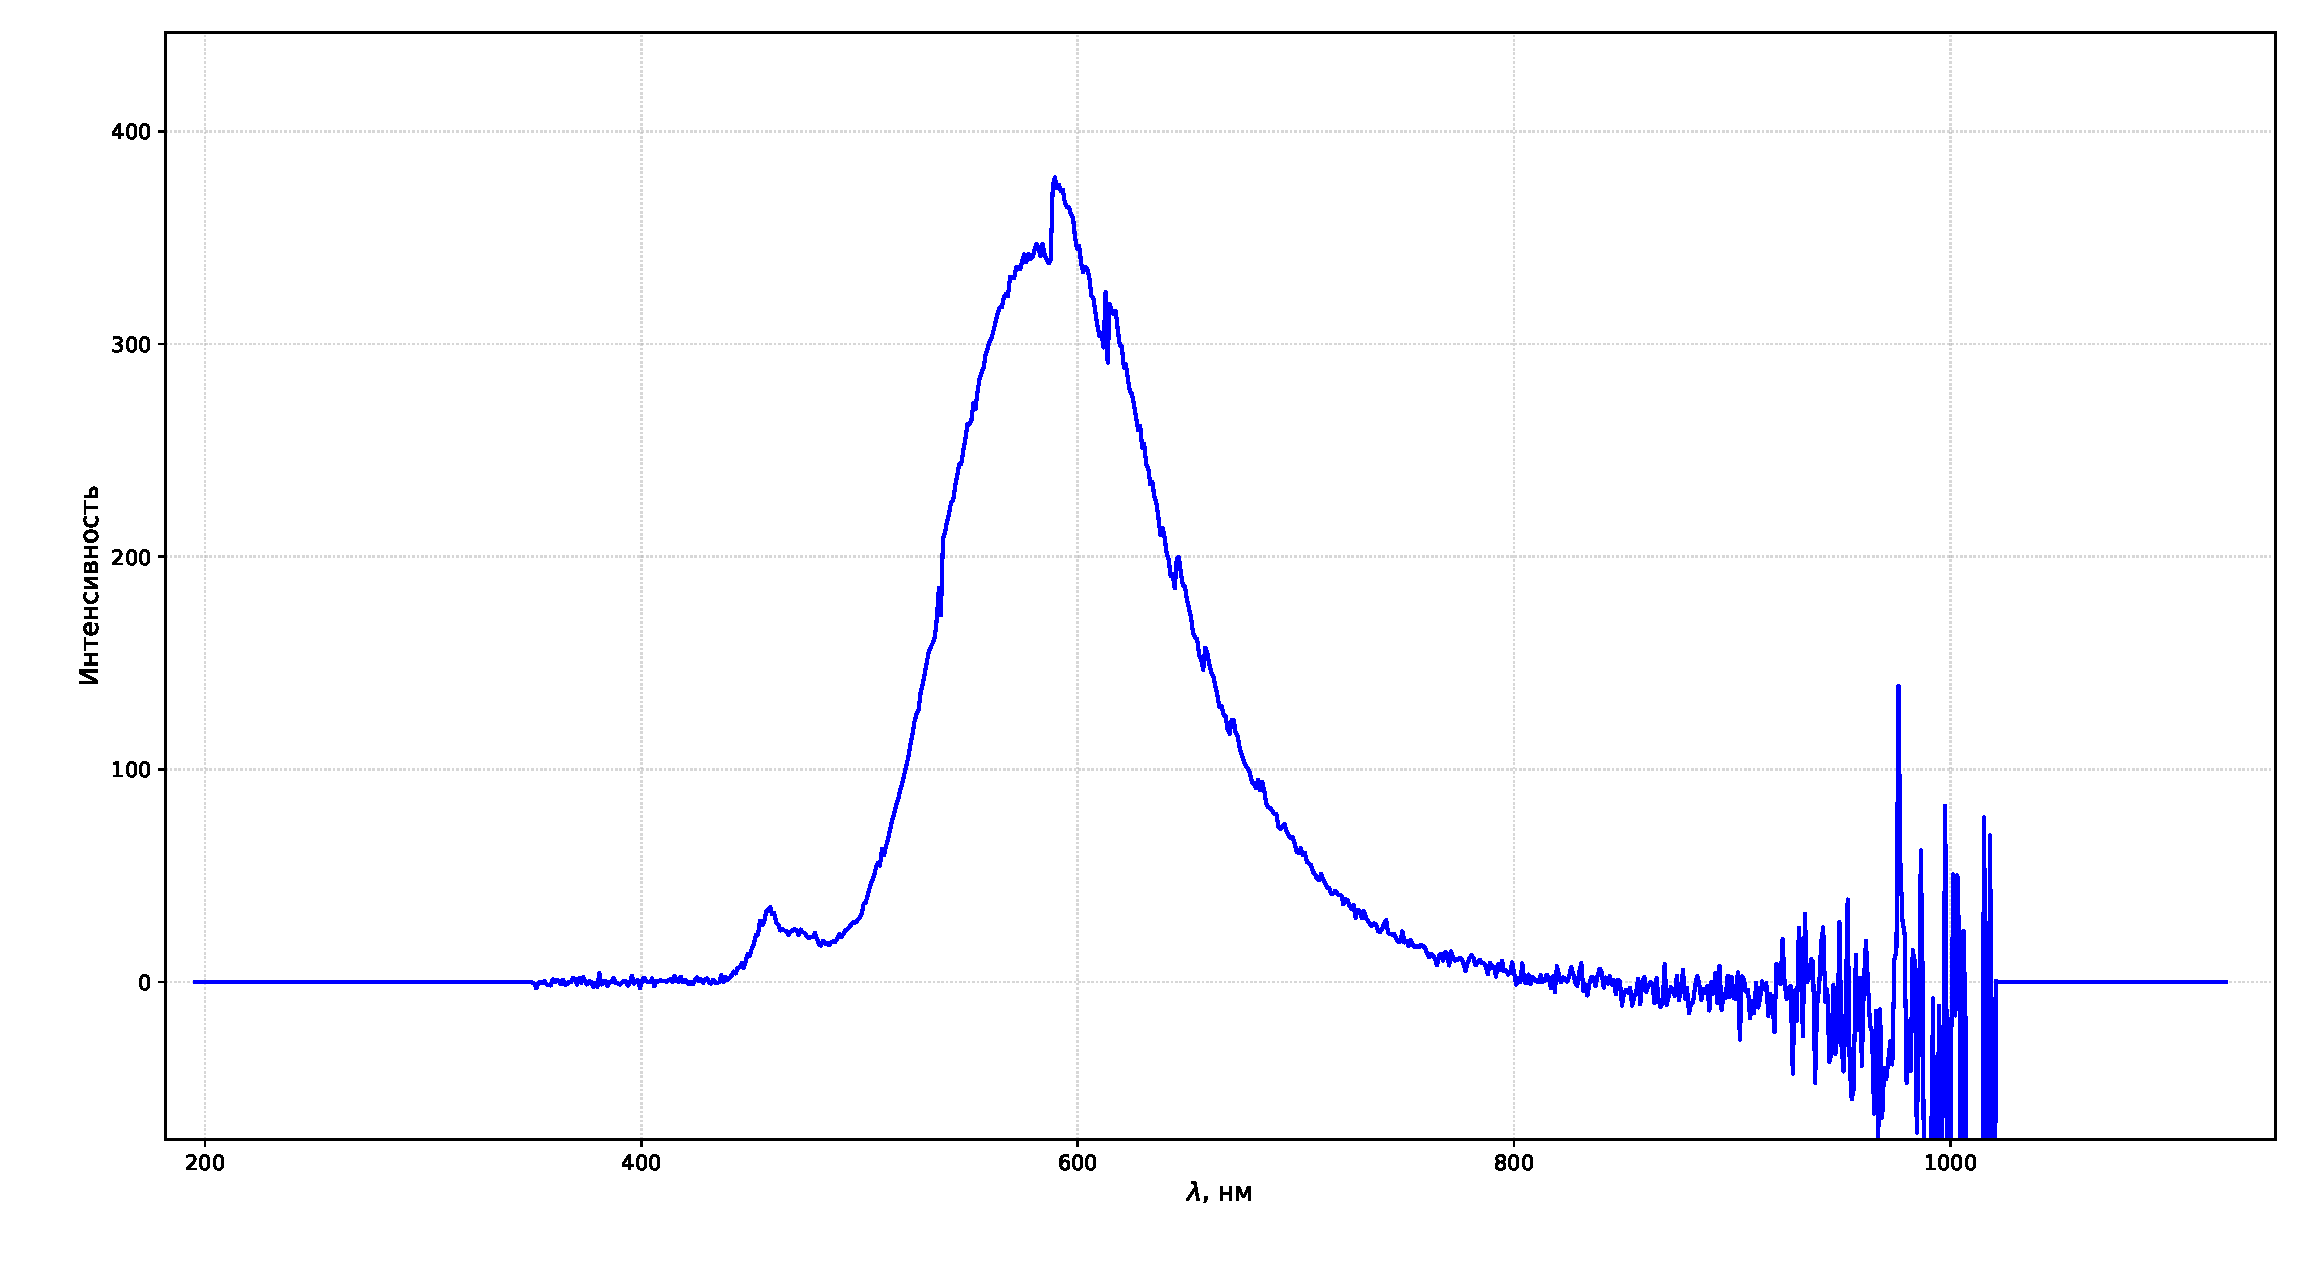
\includegraphics[width=\linewidth]{ДС5.pdf}
        \caption{Откалиброванный спектр фильтра ДС 5}
    \end{minipage}
    \hfill
    \begin{minipage}{0.48\textwidth}
        \centering
        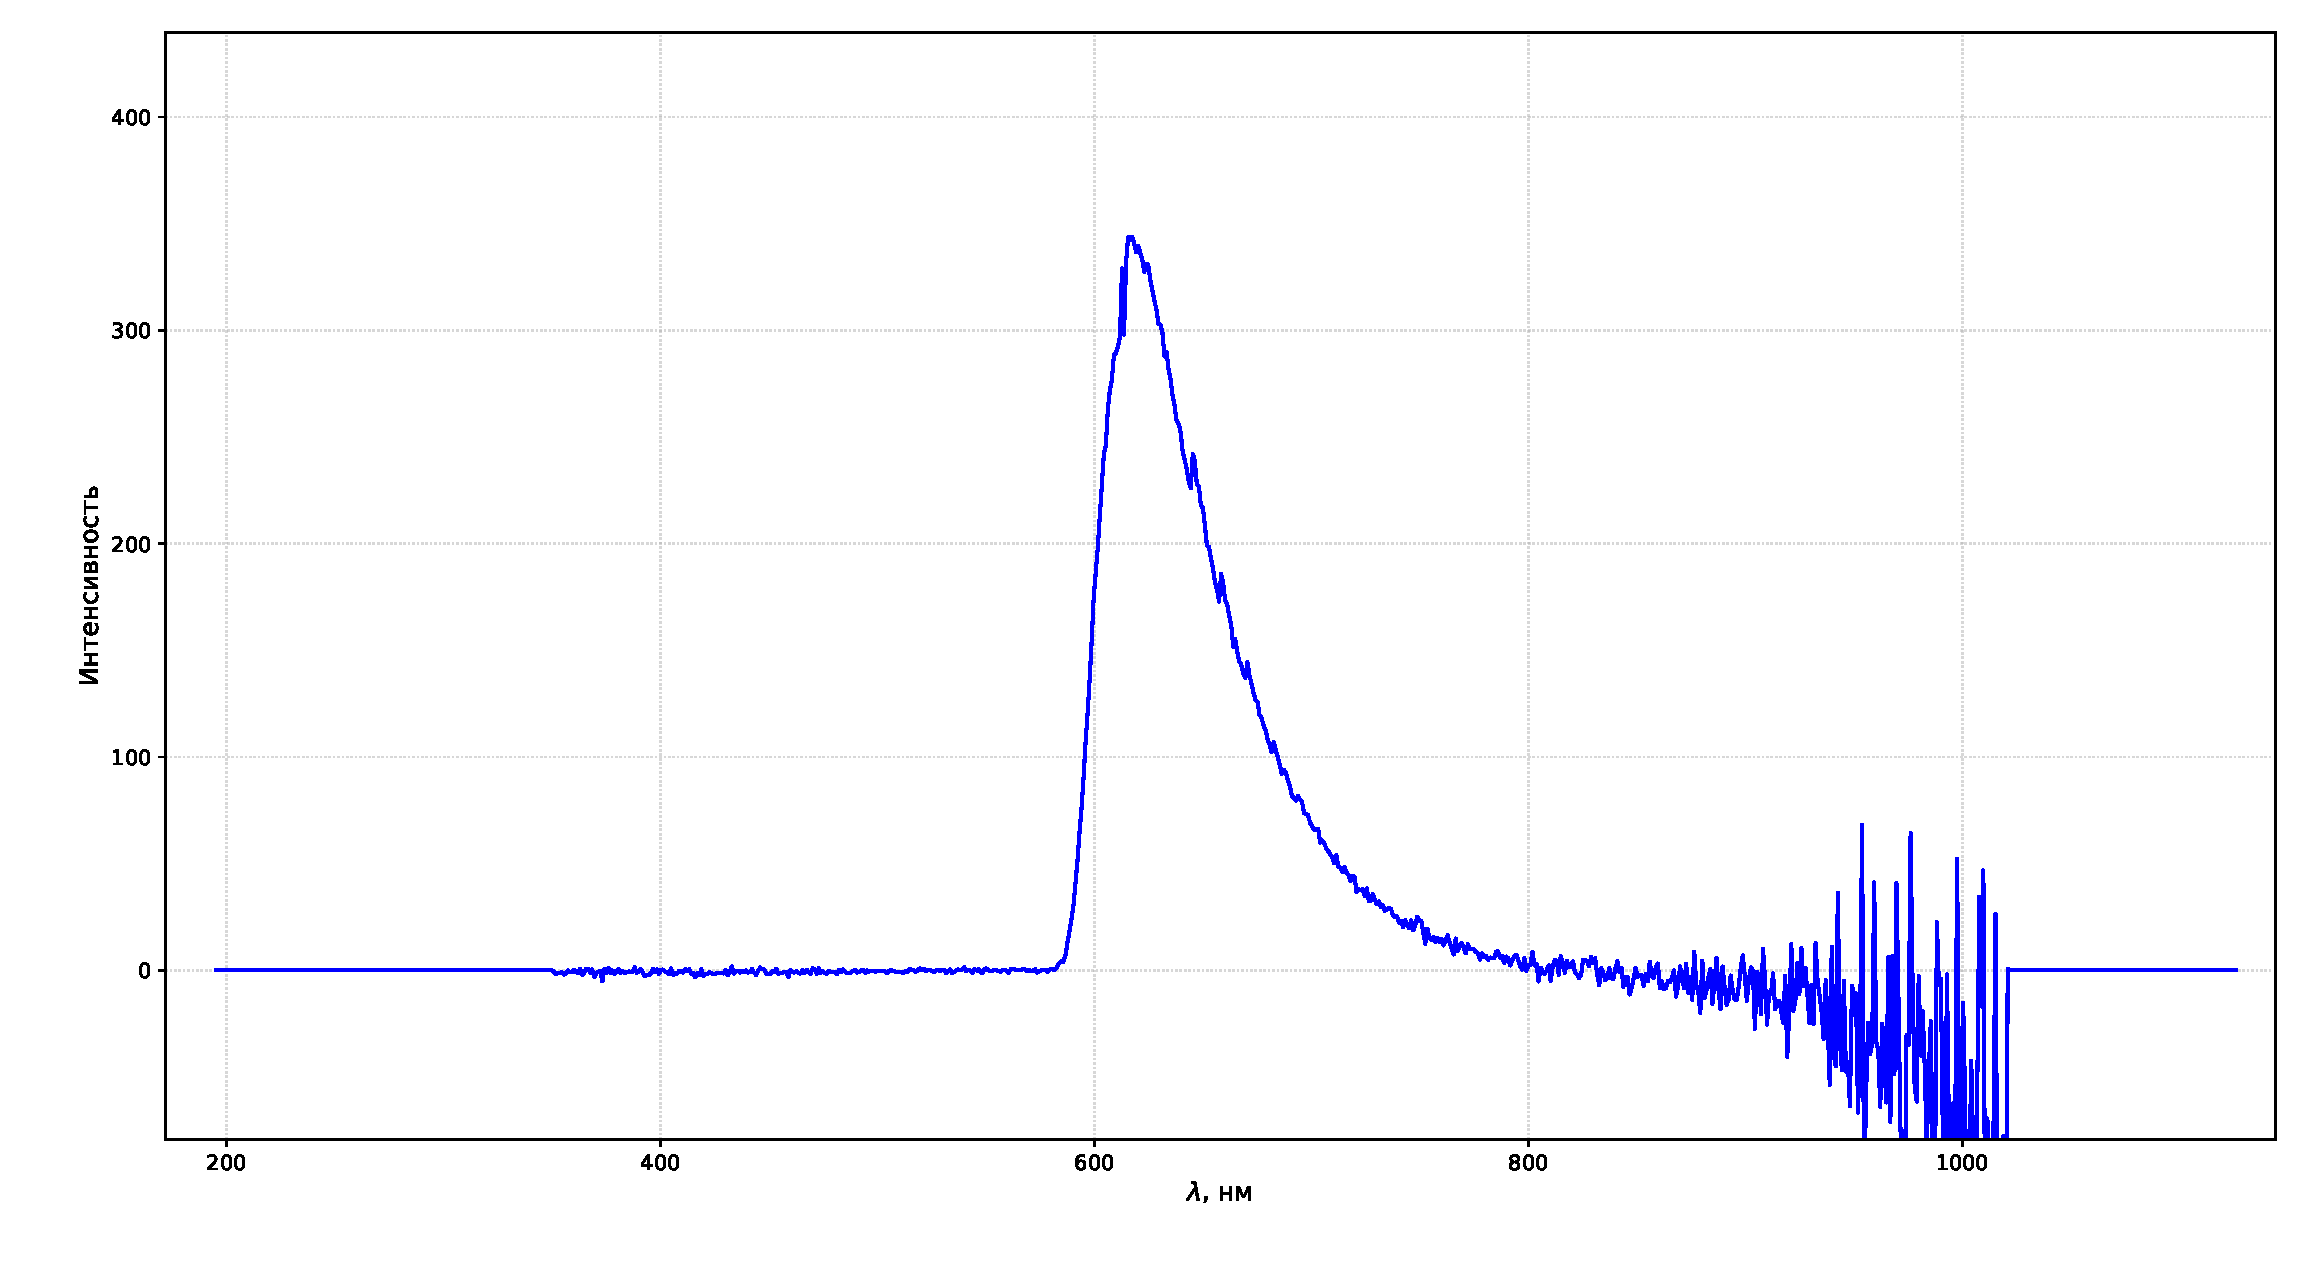
\includegraphics[width=\linewidth]{КС10.pdf}
        \caption{Откалиброванный спектр фильтра КС 10}
    \end{minipage}
\end{figure}

% Вторая пара
\begin{figure}[H]
    \centering
    \begin{minipage}{0.48\textwidth}
        \centering
        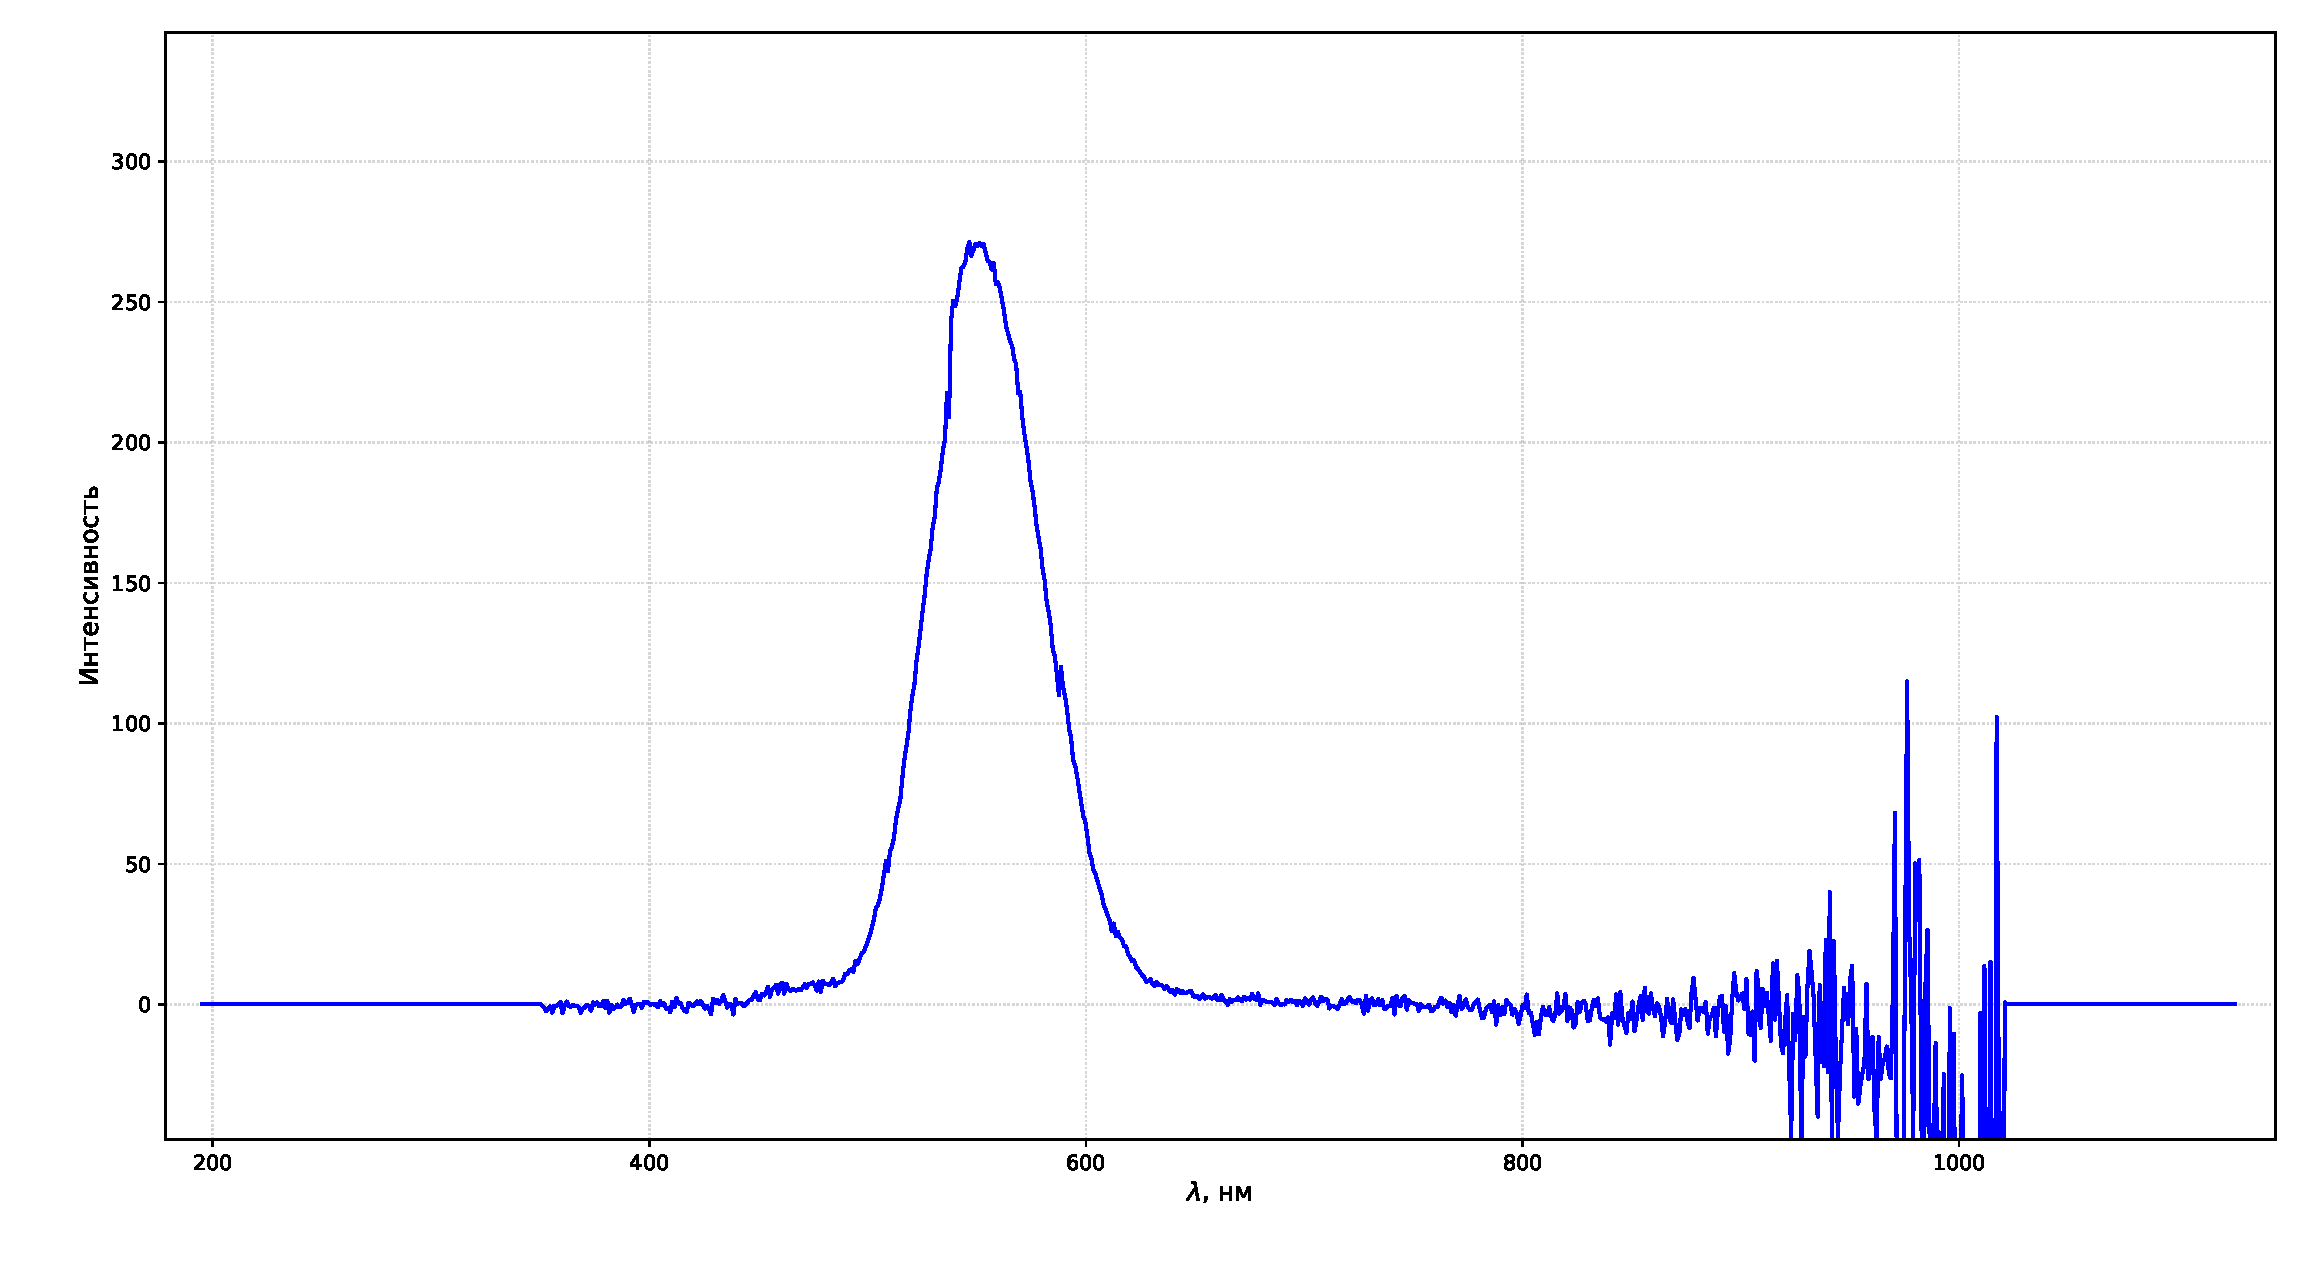
\includegraphics[width=\linewidth]{ЗС10.pdf}
        \caption{Откалиброванный спектр фильтра ЗС 10}
    \end{minipage}
    \hfill
    \begin{minipage}{0.48\textwidth}
        \centering
        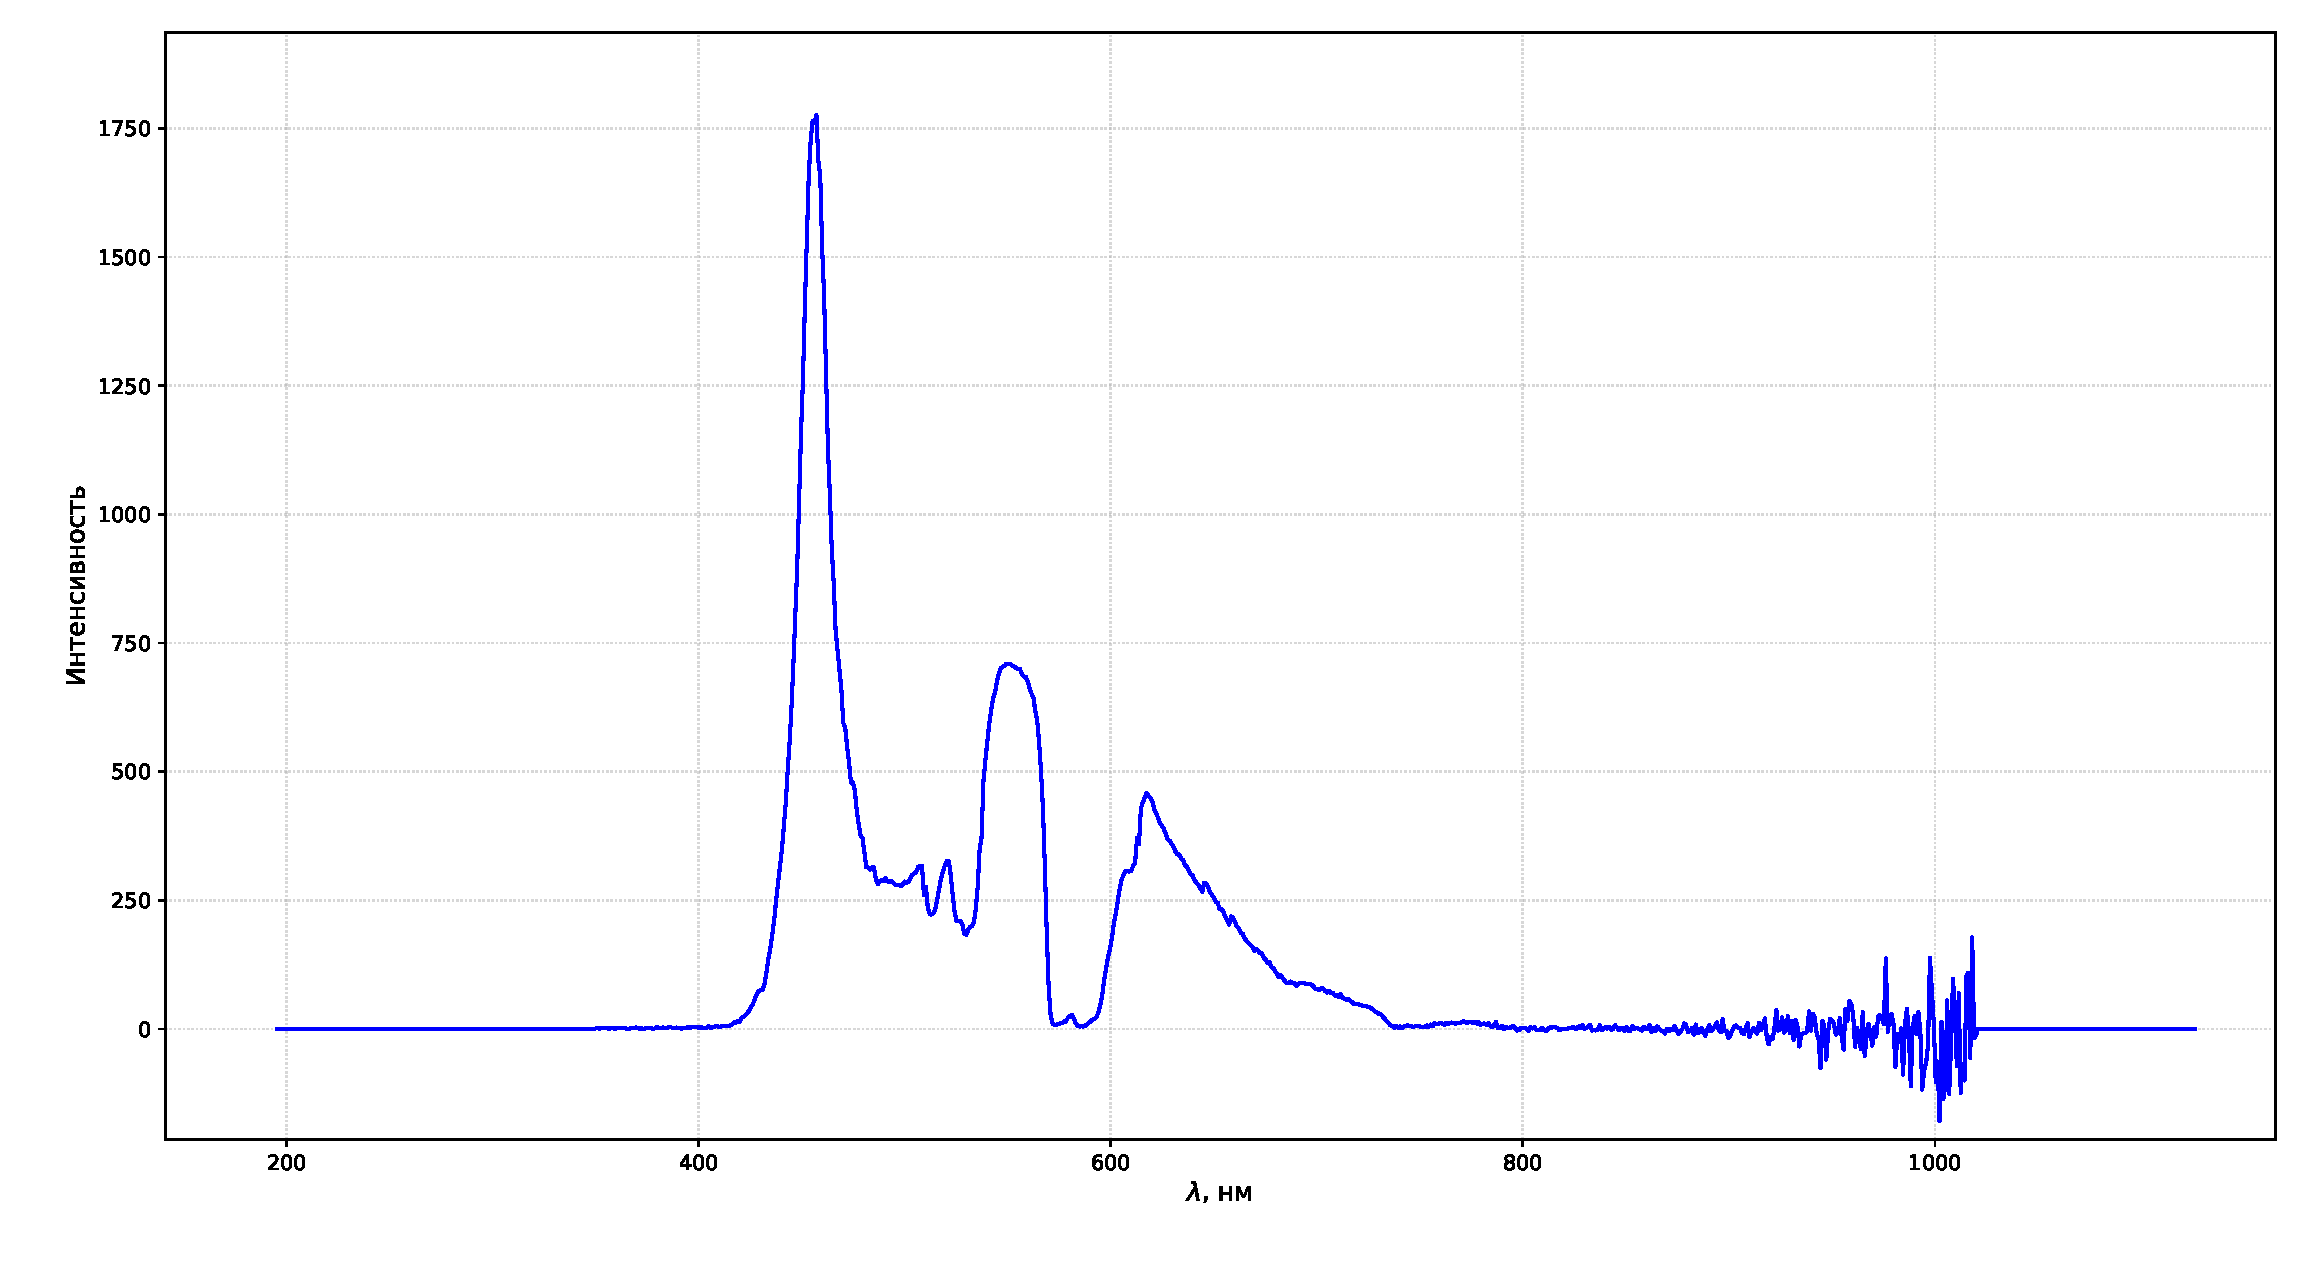
\includegraphics[width=\linewidth]{ПС7.pdf}
        \caption{Откалиброванный спектр фильтра ПС 7}
    \end{minipage}
\end{figure}

% Третья пара
\begin{figure}[H]
    \centering
    \begin{minipage}{0.48\textwidth}
        \centering
        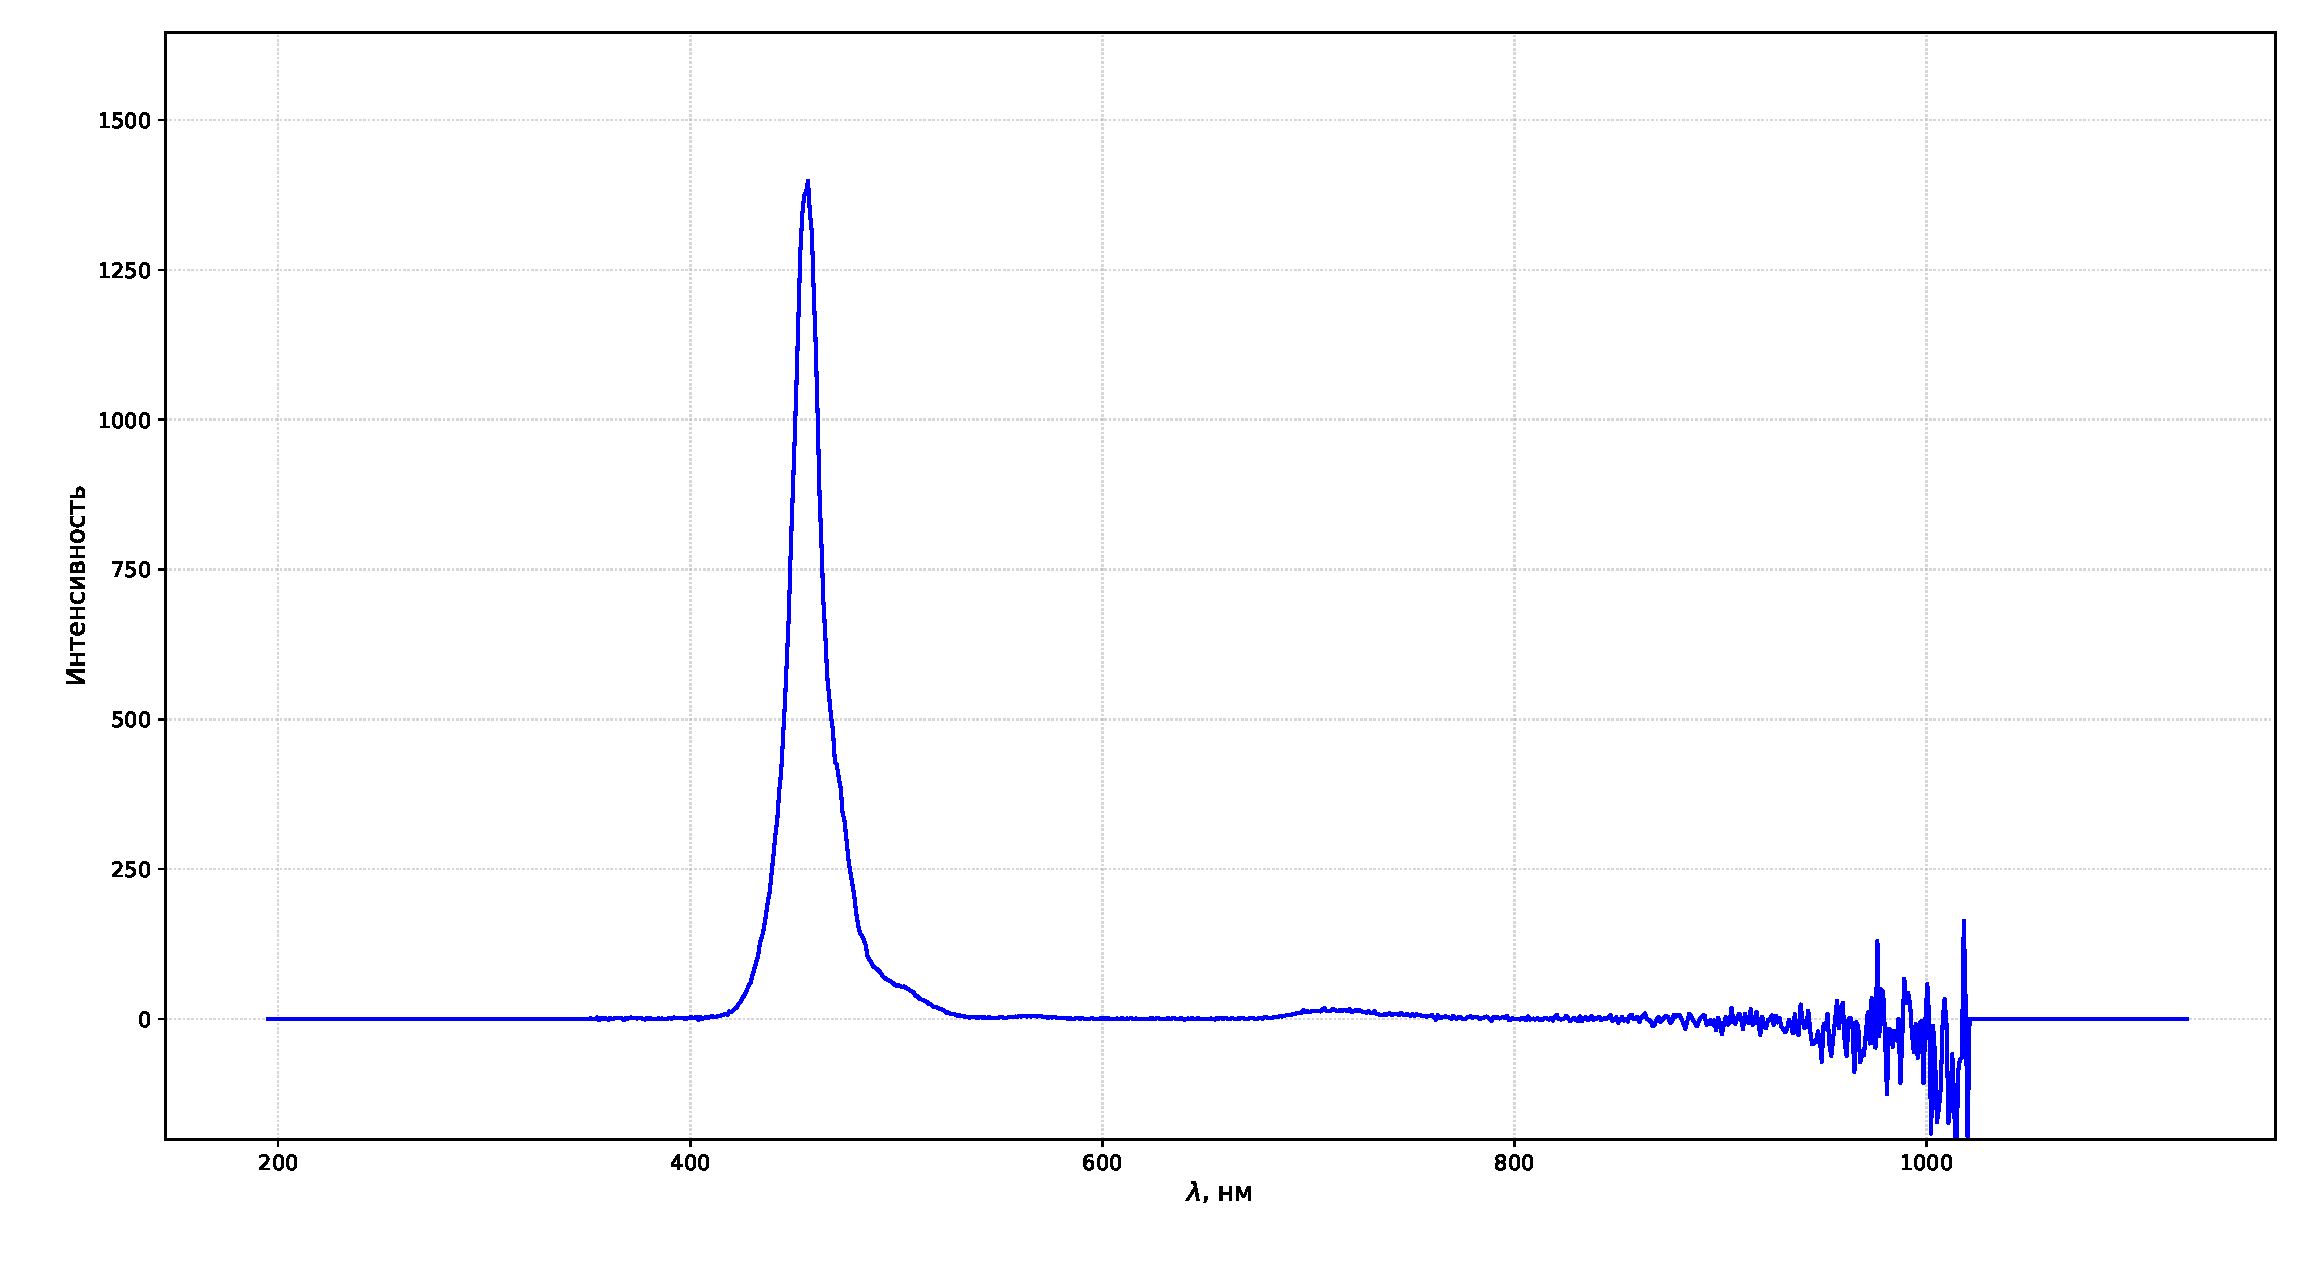
\includegraphics[width=\linewidth]{СС5.pdf}
        \caption{Откалиброванный спектр фильтра СС 5}
    \end{minipage}
    \hfill
    \begin{minipage}{0.48\textwidth}
        \centering
        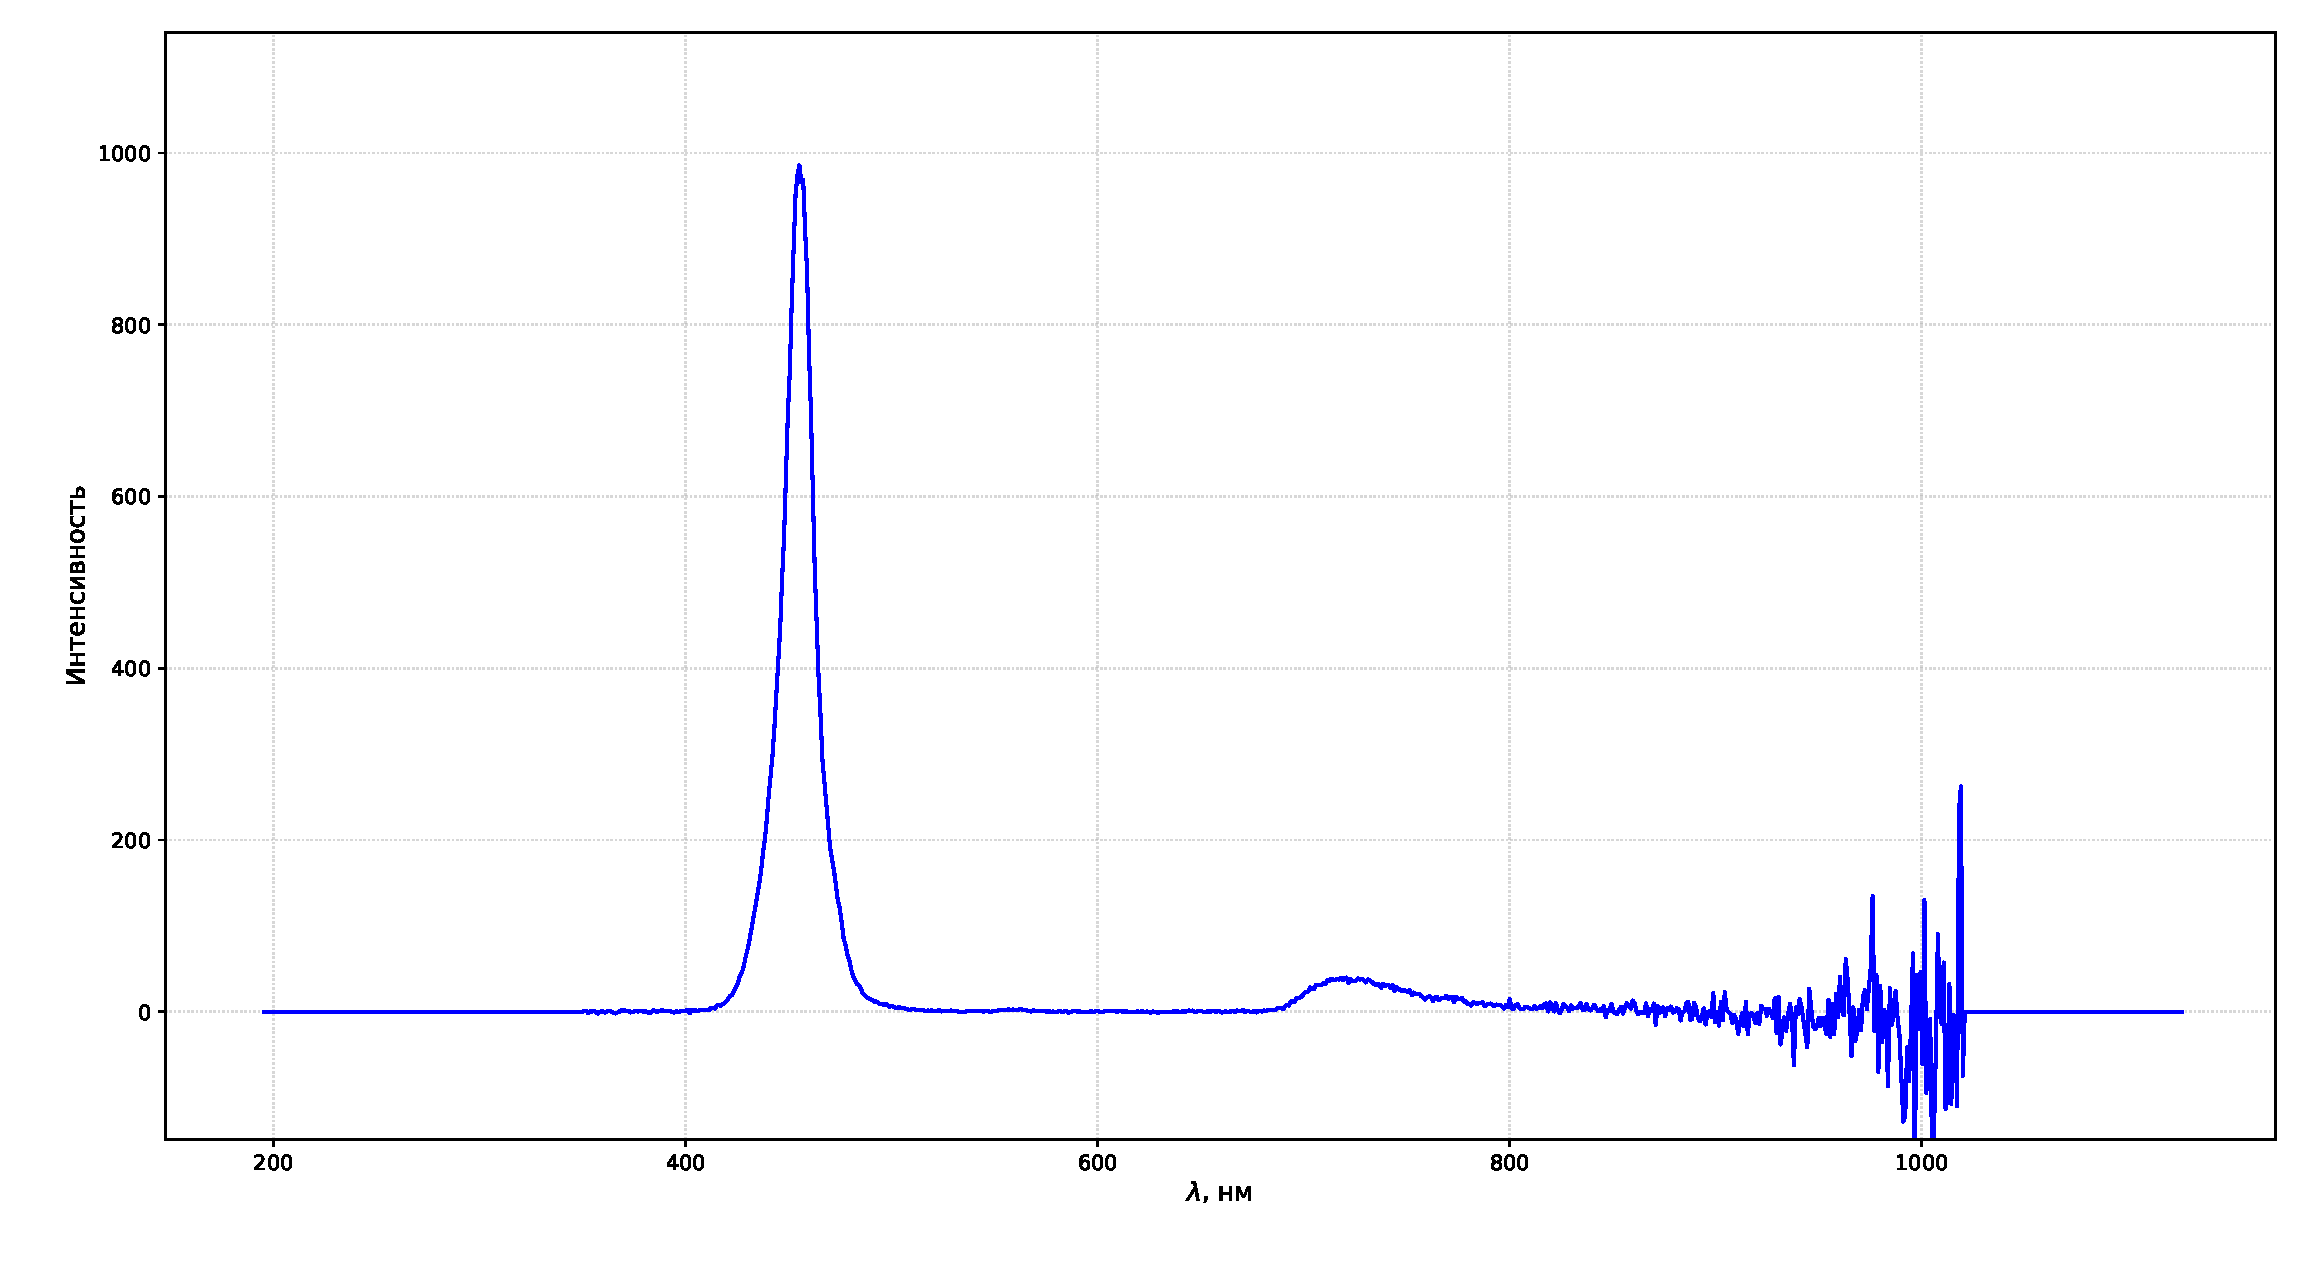
\includegraphics[width=\linewidth]{СС4.pdf}
        \caption{Откалиброванный спектр фильтра СС 4}
    \end{minipage}
\end{figure}

% Последний одиночный (ФС1)
\begin{figure}[H]
    \centering
    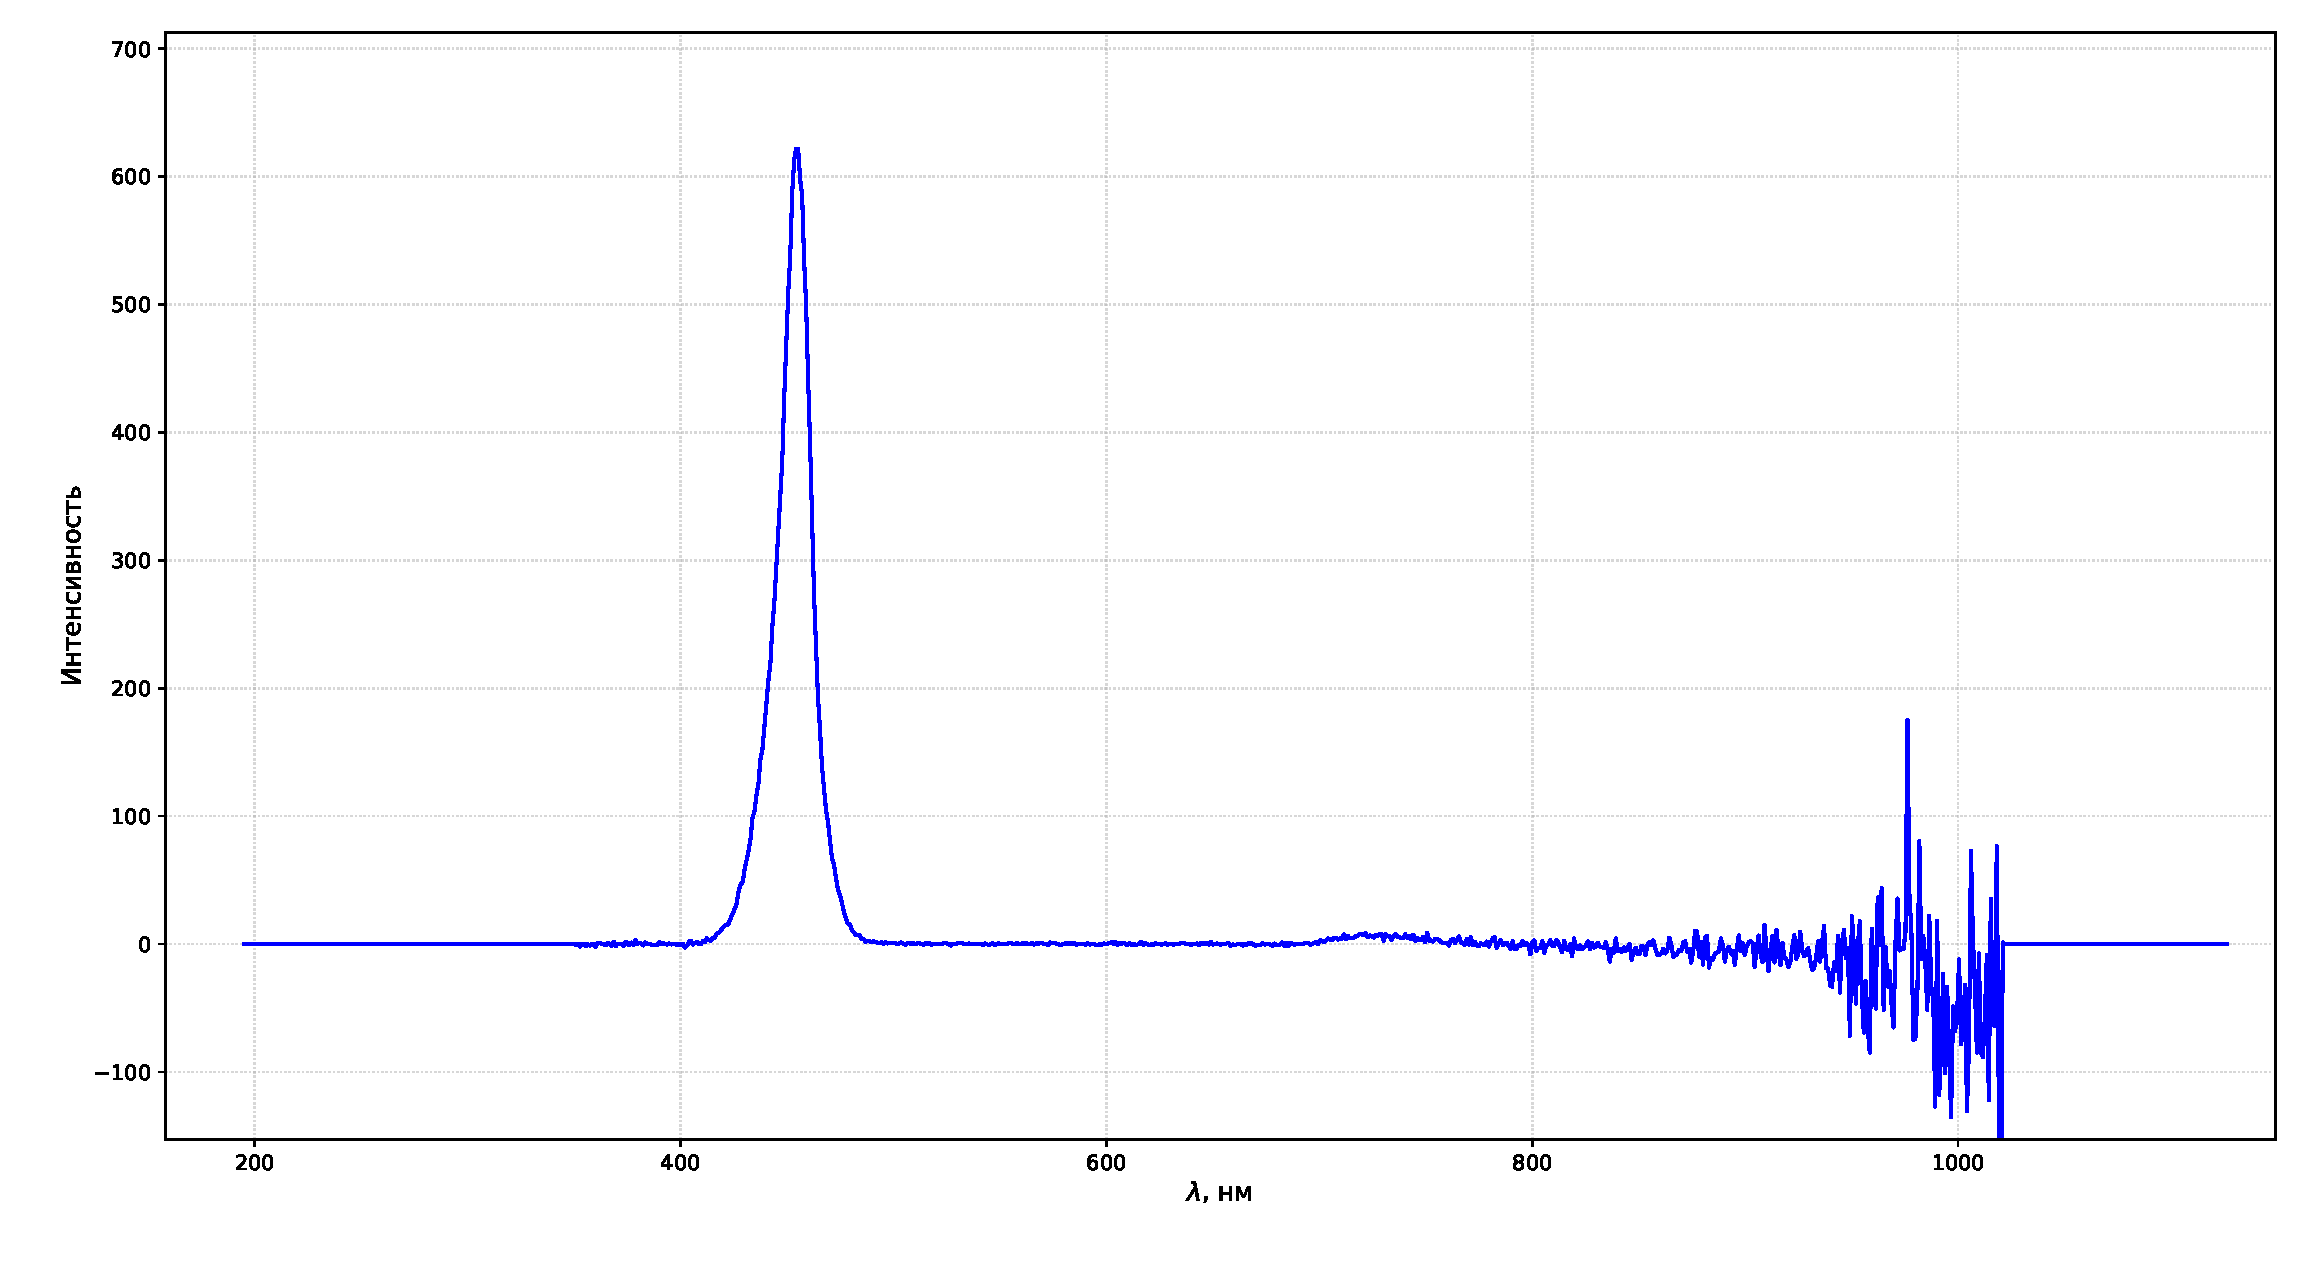
\includegraphics[width=0.48\textwidth]{ФС1.pdf}
    \caption{Откалиброванный спектр фильтра ФС 1}
\end{figure}



Полученные спектральные зависимости были проинтегрированы. Данные интегралы
пропорциональны мощности излучения, прошедшего через фильтры и падающего на
фотокатод. За k = 1 была принята самая большая площадь (для ПС 7), то есть предполагается, что это
максимум излучения, который мог пройти через фильтры.

На основании найденных коэффициентов и измеренного экранного тока с использованием
каждого из фильтров, была вычислена спектральная чувствительность катода:

\[ \Phi = \dfrac{I_{\text{экр}}}{k} \]

Данная характеристика имеет смысл только для фильтров, пропускающих только узкий диапазон. Результаты представлены в таблице 3:

\begin{table}[H]
\centering
\begin{tabular}{|c|c|c|c|c|c|}
\hline
Фильтр & Интеграл, усл. ед. & $k$ & Ток экрана $I_{\text{экр}}$, мкА & $\lambda$, нм & $\Phi$, мкА   \\ \hline
ДС 5   & 45538,09           & 0,446 & 0,898           & 582   & 2,014891 \\ \hline
КС 10  & 23551,35           & 0,230 & 0,548           & 620   & 2,377468 \\ \hline
ЗС 10  & 17364,52           & 0,170 & 0,595           & 552   & 3,501097 \\ \hline
ПС 7   & 102176,26          & 1,000 & 1,303           & --    & 1,303    \\ \hline
СС 5   & 33976,66           & 0,333 & 0,933           & 457   & 2,805763 \\ \hline
СС 4   & 23833,44           & 0,233 & 0,668           & --    & 2,863781 \\ \hline
ФС 1   & 12756,54           & 0,125 & 0,367           & 455   & 2,939566 \\ \hline
\end{tabular}
\caption{Результаты измерений по графикам}
\end{table}


Был построен график зависимости спектральной чувствительности от длины волны $\Phi(\lambda)$ (рис. 13). Видно, что качественно он совпадает с графиком теоретической спектральной чувствительности для
фотокатода S20, которая приведена на рисунке 14, где 1 - S20(UV) на MgF$_2$, 2 - S20(UV)
на кварце, 3 - широкополосный на кварце, 4 - солнечно-слепой на кварце, 5 - HOT S20 на
кварце, 6 - S20 на ВОП, 7 - Super S25 на стекле.


\begin{figure}[H]
    \centering
    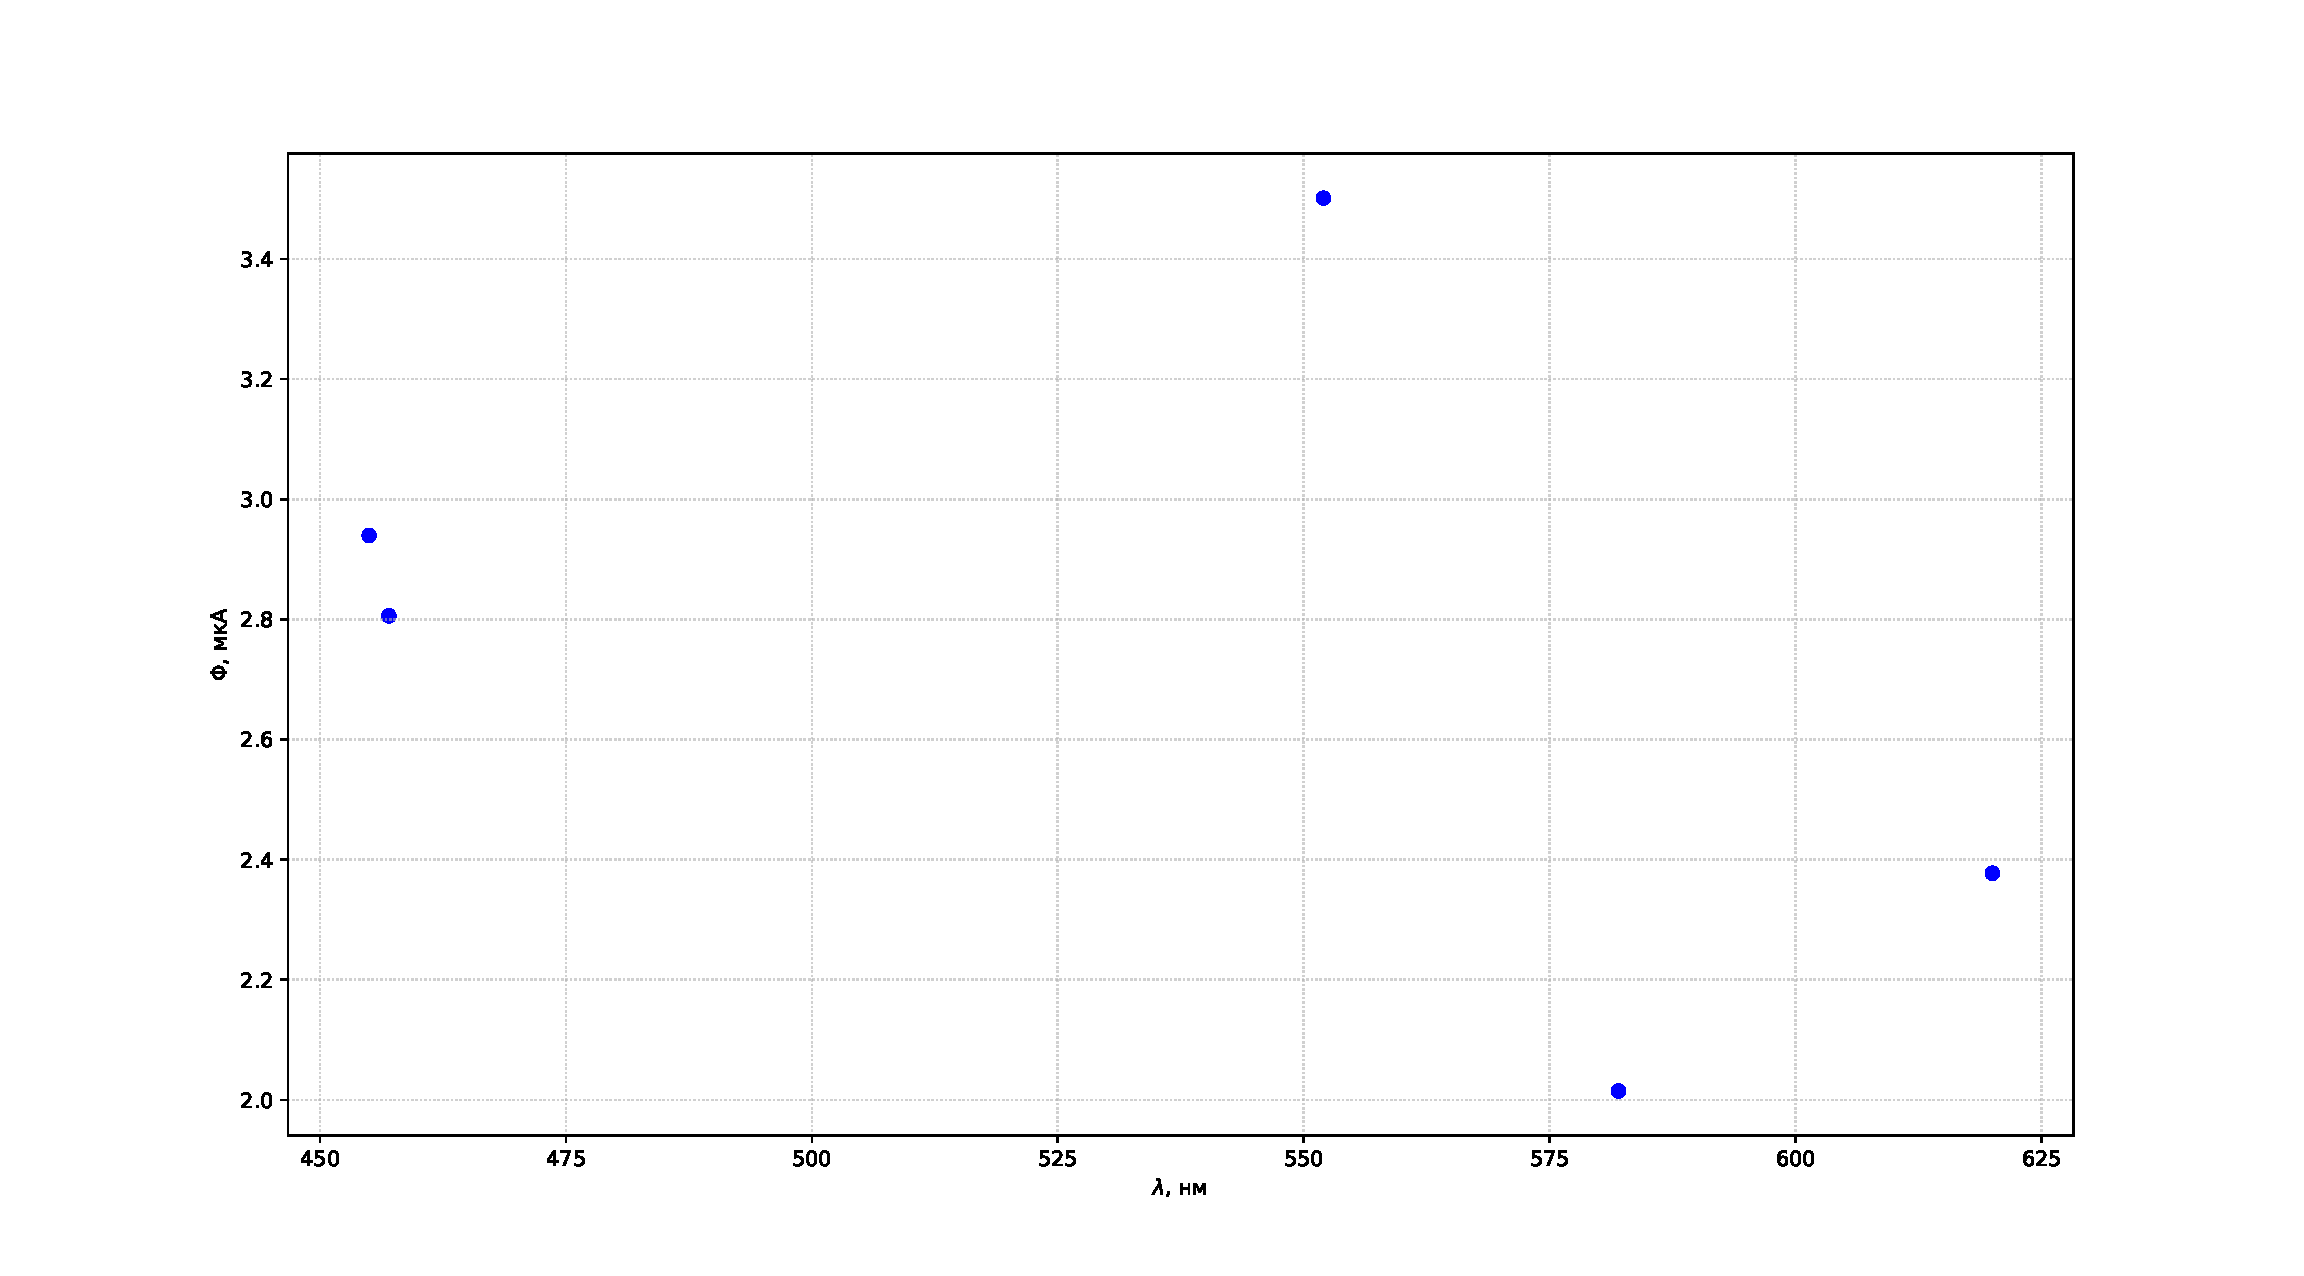
\includegraphics[width=0.7\textwidth]{Чувствительность.pdf}
    \caption{Спектральная чувствительность фотокатода в установке $\Phi(\lambda)$}
\end{figure}


\begin{figure}[H]
    \centering
    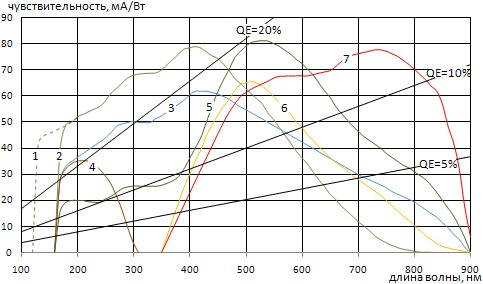
\includegraphics[width=0.7\textwidth]{С20.jpg}
    \caption{Спектральная чувствительность для фотокатода S20}
\end{figure}




\section*{Выводы}

% \begin{itemize}
%     \item В ходе работы удалось измерить зависимость коэффициента усиления МКП от напряжения - в начальном отрезке данных она совпала с экспоненциальной;
%     \item также была измерена зависимости чувствительности от длины волны для фотокатода, используемого в работе. Было проведено сравнение полученных данных с зависимостями чувствительности для фотокатодов, изготовленных из разных материалов.
% \end{itemize} 

В ходе работы удалось измерить зависимость коэффициента усиления МКП от напряжения -- в каждом промежутке при одинаковых фильтрах наблюдается экспоненциальная
зависимость, что хорошо согласуется с теорией. При снижении входящего излучения наклон графиков уменьшается.

Измерена интенсивность света при прохождении через семь различных светофильтров. Также была
измерена спектральная характеристика фотокатода для пяти длин волн. Построенная спектральная характеристика фотокатода согласуется с теоретической.

%     Проведем серию измерений. Будем при различных значениях напряжения на микроканальной пластине измерять ток на катоде и ток на экране. Ток на экране будет больше тока на катоде, поскольку микроканальная пластина "умножила"\ падающие на нее электроны. Соответственно, коэффициент усиления -- то, во сколько раз ток после пластины стал больше -- вычисляется по формуле (\ref{formula_k_I}). Однако, из-за особенностей проектирования установки ток на катоде будет ненулевым, даже если фотоны не падают на фотокатод. Значит, закроем входное отверстие установки, чтобы в нее не попадал свет, и измерим нулевой ток на катоде $I_{катод}^0$(при различных $U_{мкп}$). Отнормируем на эту величину значения токов на катоде(формула (\ref{formula_I_cathode})), получившуюся величину обозначим $I_{катод}^\Sigma$. Итоговые результаты измерений представлены в таблице \ref{table_multi_coef}.

%     \begin{table}[H]
%     \centering
%     \begin{tabular}{|c|c|c|c|c|c|}
%     \hline
%         № & 1 & 2 & 3 & 4 & 5 \\ \hline
%         $I_{катод},\ мкА$ & 0,0049 & 0,0051 & 0,0053 & 0,0056 & 0,0058 \\ \hline
%         $U_{мкп},\ кВ$ & 0,5846 & 0,668 & 0,729 & 0,8143 & 0,8906 \\ \hline
%         $I_{экран},\ мкА$ & 0,0123 & 0,0638 & 0,1775 & 0,6273 & 1,3026 \\ \hline
%         $I_{катод}^0,\ мкА$ & 0,0021 & 0,0024 & 0,0025 & 0,0028 & 0,003 \\ \hline
%         $I_{катод}^\Sigma,\ мкА$ & 0,0028 & 0,0027 & 0,0028 & 0,0028 & 0,0028 \\ \hline
%         $k$ & 4,393 & 23,630 & 63,393 & 224,036 & 465,214 \\ \hline
%     \end{tabular}
%     \caption{Результаты измерения параметров установки при различных напряжениях на МКП.}
%     \label{table_multi_coef}
%     \end{table}

%     % \begin{figure}[H]
%     %     \centering
%     %     \includegraphics[width=1\linewidth]{images/k(U).png}
%     %     \caption{График зависимости $k(U_{мкп})$.}
%     %     \label{img_k_I(U)}
%     % \end{figure}

% \subsection*{Измерение коэффициента усиления МКП по яркости.}

%     При каждом значении напряжения $U_{мкп}$ будем делать фотографию экрана. Выберем любую секцию между прутьями сетки и будем измерять в ней среднюю яркость $\langle B_{центр}\rangle$ в некоторых условных единицах. Однако, темный фон также имеет некоторую яркость, измерим среднее значение яркости фона $\langle B_{фон}\rangle$. Найдем значение относительной средней яркости изображения $\langle B_{отн}\rangle$ по формуле (\ref{formula_B}).\par
%     Далее будем модулировать яркость изображения коэффициентом усиления по току, т.е будем считать, что при $\langle B_{отн}\rangle = 6,863$ коэффициент усиления по яркости равен коэффициенту усиления по току $k = 4,393$, а все остальные значения $\langle B_{отн}\rangle$ будем пересчитывать по формуле (\ref{formula_k_B}). Результаты измерений и расчетов представлены в таблице \ref{table_B}.
    
%     \begin{table}[!ht]
%     \centering
%     \begin{tabular}{|c|c|c|c|c|c|}
%     \hline
%         № & 1 & 2 & 3 & 4 & 5 \\ \hline
%         $U_{мкп},\ кВ$ & 0,5846 & 0,668 & 0,729 & 0,8143 & 0,8906 \\ \hline
%         $\langle B_{центр}\rangle,\ у.е$ & 25,336 & 63,473 & 106,109 & 139,791 & 132,955 \\ \hline
%         $\langle B_{фон}\rangle,\ у.е$ & 18,473 & 18,722 & 18,939 & 19,401 & 19,962 \\ \hline
%         $\langle B_{отн}\rangle,\ у.е$ & 6,863 & 44,751 & 87,17 & 120,39 & 112,993 \\ \hline
%         $k$ & 4,393 & 28,644 & 55,796 & 77,059 & 72,324 \\ \hline
%     \end{tabular}
%     \caption{Результаты измерения яркости изображения при различных $U_{мкп}$.}
%     \label{table_B}
%     \end{table}

%     Изобразим результаты на графике зависимости $k(U)$ совместно с результатами предыдущего эксперимента.

%     % \begin{figure}[H]
%     %     \centering
%     %     \includegraphics[width=1\linewidth]{images/k(U)_joint.png}
%     %     \caption{График зависимости $k(U_{мкп})$.}
%     %     \label{img_k_B(U)}
%     % \end{figure}

% \subsection*{Исследование спектральной чувствительности МКП.}
%     При постоянном напряжении на микроканальной пластине $U_{мкп} = 0,8848\ кВ$ измерим коэффициент усиления по току для разных длин волн света, попадающего на фотокатод. Результаты измерений представлены в таблице \ref{table_integral}. Построим спектры пропускания используемых для выделения этих длин волн светофильтров и откалибруем их. Результаты представлены на рис.\ref{img_spectrum}.

%     % \begin{figure}[h]  
%     % \vspace{2ex} 
%     % \centering 
%     % \subfigure[]
%     % {
%     %     \includegraphics[width=0.5\linewidth]{images/spectrum_noncaibrated.png} \label{img_spectrum_noncalibrated} 
%     % }  
%     % \hspace{-8ex}
%     % \subfigure[]
%     % {
%     %     \includegraphics[width=0.5\linewidth]{images/spectrum_caibrated.png} \label{img_spectrum_calibrated} 
%     % } 
%     % \caption{Спектры пропускания светофильтров: 
%     %     \subref{img_spectrum_noncalibrated} некалиброванные; \subref{img_spectrum_calibrated} калиброванные. }
%     % \label{img_spectrum}
%     % \end{figure}

%     Проинтегрируем графики интенсивности(рис.\ref{img_integral}).

%     % \begin{figure}[H]
%     %     \centering
%     %     \includegraphics[width=0.9\linewidth]{images/intensivity_integrals.png}
%     %     \caption{График зависимости $\int_0^{\lambda} I(\lambda)$.}
%     %     \label{img_integral}
%     % \end{figure}

    
%     \begin{table}[H]
%     \centering
%     \begin{tabular}{|c|c|c|c|c|}
%     \hline
%         Светофильтр  & \textsl{ЖЗС1} & \textsl{ОС14} & \textsl{УФС1} & \textsl{без} \\ \hline
%         $\lambda_{пропуск}$ & 540 & 600 & 450 & $\sim$ 550 \\ \hline
%         $I_{катод},\ мкА$ & 0,0034 & 0,0033 & 0,0038 & 0,004 \\ \hline
%         $U_{мкп},\ кВ$ & 0,8848 & 0,8848 & 0,8848 & 0,8848 \\ \hline
%         $I_{экран},\ мкА$ & 0,089 & 0,1335 & 0,377 & 0,5526 \\ \hline
%         $I_{катод}^\Sigma,\ мкА$ & 0,0005 & 0,0004 & 0,0009 & 0,0011 \\ \hline
%         $k$ & 178,00 & 333,75 & 418,89 & 502,36 \\ \hline
%         $\int_0^{\lambda_{max}} I,\ у.е\cdotнм$ & 25281,65 & 46798,02 & 11918,75 & - \\ \hline
%     \end{tabular}
%     \caption{Результаты измерения параметров при различных длинах волн падающего света.}
%     \label{table_integral}
%     \end{table}




        
% \section*{Обсуждение результатов.}    
%     Как видно из рис.\ref{img_k_I(U)} зависимость коэффициента усиления МКП по току от напряжения действительно экспоненциальная, что согласуется с теоретическими представлениями об устройстве микроканальной пластины.\par При измерении коэффициента усиления по яркости получен аномальный результат: при увеличении напряжения коэффициент усиления сначала закономерно растет и даже совпадает с коэффициентом усиления по току(см. рис.\ref{img_k_B(U)}), однако затем замедляет рост, а после и вовсе начинает уменьшаться. Мы связываем данное явление c тем, что измерение яркости производилось с помощью камеры, а она, как известно, может автоматически перенастраивать экспозицию кадра, чтобы получать более качественное изображение. Т.е на самом деле яркость увеличивалась, но в один момент увеличилась настолько, что камера автоматически сменила настройки и искусственно "затемнила"\ кадр.\par
%     В части работы, связанной с исследованием спектральной чувствительности, получены необходимые данные, однако их обработка не представляется возможной в виду отсутствия адекватного описания обработки результатов к работе.

% \section*{Выводы}


\end{document}
